\chapter{Combinations of top quark mass measurements}
\label{chap:combinations}
%
Alongside a thorough analysis of systematic uncertainties to constrain their impact on a measurement, a sizeable precision gain can be obtained by a combination of measurements. With ever-increasing precision of single experiment \tquark\ mass analyses, this approach becomes more and more promising, because the absolute precision gain of refined techniques in both theory and experiment tends to saturate. 
%
A combination of measurements requires a precise matching of uncertainty categories and a detailed evaluation of the correlations of observables. 

This chapter gives an overview of \tquark\ mass combinations and presents the combination of the analyses in the \ttbarll\ and the \ttbarlj\ channel at a \cme\ of $\sqrts=7$~\TeV. 
%
Subsequently, the measurement in the \ttbarll\ channel at a \cme\ of $\sqrts=8$~\TeV\ is combined with the $\sqrts=7$~\TeV\ analyses.
%
The status and prospects of the \gls{ATLAS} and \gls{CMS} \mt\ combination effort are discussed in \reference~\cite{Top2015combinissues}.



















\section{Previous combinations}
\label{sect:prevcomb}
%
Traditionally, combinations of top quark mass measurements are based on an a posteriori combination of published measurements. 
%
Various analysis differences like the choice of \gls{MC} simulation programs, uncertainty categorisation and analysis approaches make a precise determination of correlations impossible.
%
Therefore, the correlations of uncertainty categories are assigned based on physics arguments and varied within a reasonable range to assess the stability of the combination. This is in many cases the only possible way of combination, especially for older measurements, where the information on the specific analysis is limited to the published material.

%, since personnel fluctuation in particle physics is generally high and access to analysis details is cut off. 
%
In the last years, \gls{ATLAS}, \gls{CMS}, \gls{CDF} and \gls{D0} have therefore started to publish information relevant for a subsequent combination alongside the actual measurement. This includes, for example, the publication of detailed components of the \gls{JES} uncertainties. In addition, the \gls{ATLAS} and \gls{CMS} collaborations move towards a harmonisation of uncertainty categorisation, for example of the \gls{JES} components~\cite{ATL-PHYS-PUB-2014-020}. This facilitates the matching of uncertainty categories and leads to a more reliable correlation estimate. 

% %hadronisation uncertainty ATLAS vs CMS
% An outstanding issue with respect to harmonisation of uncertainty categories between \gls{CMS} and the other experiments is the treatment of the uncertainty related to parton shower and hadronisation effects, commonly denoted as hadronisation uncertainty. Traditionally, it is estimated from the observed mass difference of two parton shower generators, covering different parton shower concepts (\pt\ ordered or angular ordered), fragmentation functions, tunes and the difference of the cluster and string hadronisation models. Undoubtedly, this introduces a certain amount of double-counting with the \gls{JES} and \gls{bJES} uncertainties. However, the extent of this is at present unknown and under debate. 
% %
% The \gls{CMS} collaboration avoids all double-counting and does not quote an explicit hadronisation uncertainty, assuming that the effects are fully covered by alternative uncertainties. These are a flavour dependent hadronisation uncertainty and an uncertainty covering variations of the $b$-fragmentation, \bhadron\ branching fractions and \tquark\ \pt\ modelling~\cite{Khachatryan:2015hba}.
% %
% The \gls{ATLAS} and the Tevatron collaborations take the conservative approach and quote the full difference of two samples with different parton shower generator as uncertainty. The assumption, that the \gls{JES} uncertainties do not cover the effect, is motivated by the event topology differences of the \ttbar\ events, from which the impact on the \mt\ measurement is evaluated, and the dijet and \Zboson\ events, from which the \gls{JES} uncertainty is determined. A recent study from \gls{ATLAS} shows that the amount of double-counting is indeed small~\cite{ATL-PHYS-PUB-2015-042}.
% %
% Due to the relatively large impact of this uncertainty on different analyses of $\order(0.5)~\GeV$, a common treatment of this uncertainty is of high importance. Studies and intense discussions to resolve this issue are ongoing. 




%world combination
Setting aside categorisation differences~\cite{Top2015combinissues}, combinations of results of all four experiments have been performed. The world combination, including 11 measurements from Tevatron and \gls{LHC}~\cite{ATLAS:2014wva}, is shortly described here. It serves as showcase for the standard combination approach, used for example for the \gls{LHC}~\cite{LHC2013}, the Tevatron~\cite{TEWG2014} and the former \gls{CMS}~\cite{CMS-PAS-TOP-14-015} combinations. The recent \gls{CMS} combination has been performed with a so-called reduced correlation scenario, based on a redefinition of correlations as uncertainty ratios~\cite{Khachatryan:2015hba}. A critical assessment of this method is given in \reference~\cite{BLUERN}.

The world combination includes measurements performed by the \gls{CDF} and \gls{D0} experiments at the Tevatron and the \gls{ATLAS} and \gls{CMS} experiments at the \gls{LHC}. 
%
The Tevatron measurements are based on up to $\intlumi=8.7~\invfb$ of proton--anti-proton collisions, recorded at a \cme of $1.96~\TeV$. 
%
The \gls{LHC} data used for this combination correspond to $\intlumi=4.9~\invfb$ of \pp\ collision data, recorded at a \cme of $7~\TeV$. 
%
\gls{CMS} and \gls{CDF} contribute a measurement in each of the three main \ttbar\ decay channels. \gls{CDF} provides a measurement in the \met+jets channel in addition. \gls{ATLAS} and \gls{D0} contribute two measurements each, one in the \ttbarll\ and one in the \ttbarlj\ channel. The input measurements and the combination results are shown in \fig~\ref{fig:worldcombisummary}.
%
%
%%%%%%%%%%%%%%%%%%%%%%%%%%%%%%%%%%%%%%%%%%%%%%%%%%%%%%%%%%%%%%%%%%%%%%%%%%%%%%%
\begin{figure*}[tbp!]
\centering
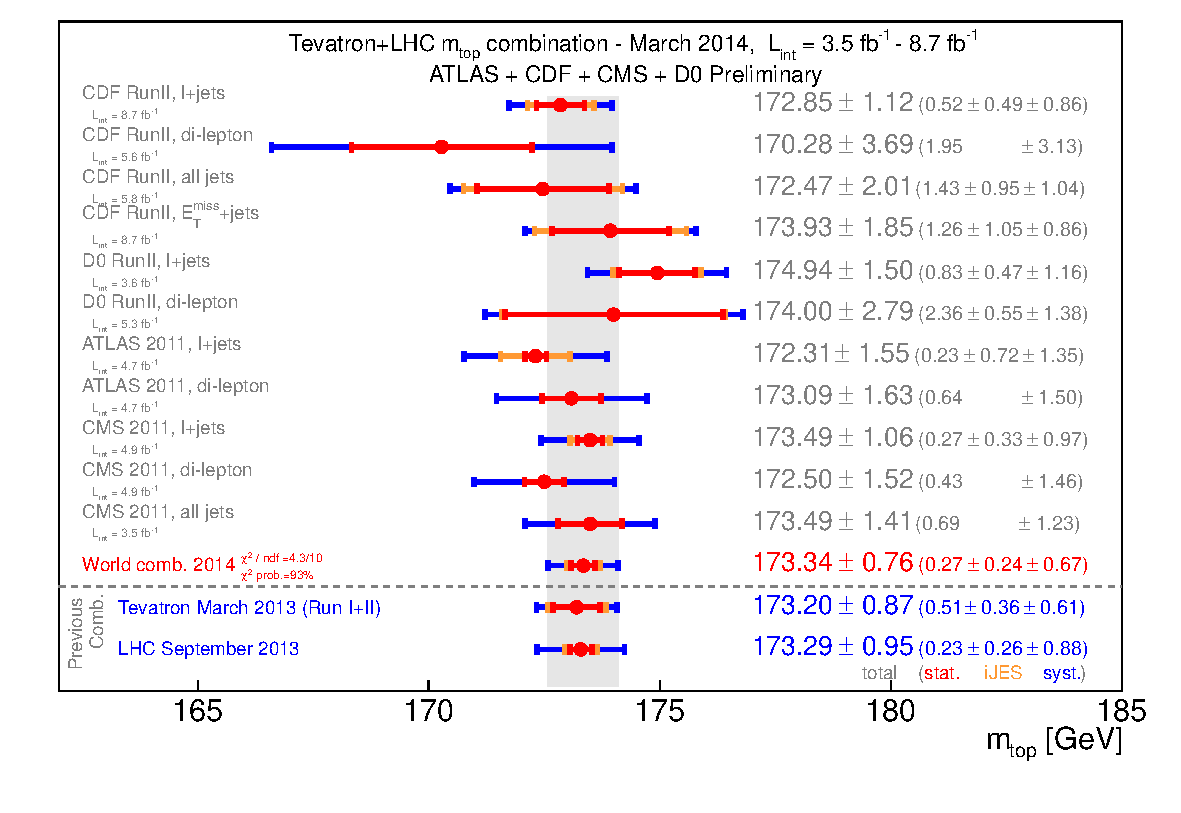
\includegraphics[width=0.8\textwidth]{./figs/world_combi_summary.pdf}
\vspace{-0.5cm}
\caption[\Tquark\ mass world combination]{
%
The input measurements and the result of the world combination of Tevatron and \gls{LHC} experiments. The \gls{ATLAS} input measurements~\cite{ATLAS-CONF-2013-046,ATLAS-CONF-2013-077} are now superseded by \reference~\cite{Aad:2015nba}.
%
\label{fig:worldcombisummary}
}
\end{figure*}
%%%%%%%%%%%%%%%%%%%%%%%%%%%%%%%%%%%%%%%%%%%%%%%%%%%%%%%%%%%%%%%%%%%%%%%%%%%%%
%
%
The combination is performed using the \gls{BLUE} method~\cite{BLUE1,BLUERN} in a \Cpp\ implementation described in \reference~\cite{BLUEcpp}.
%
The \gls{BLUE} method combines two or more measurements based on a linear combination of the inputs. 
%
The coefficients are determined via the minimisation of the total variance of the combined result. They can be used to construct measures for the importance of a given single measurement in the combination. 
%
The central values, the list of uncertainty components and the correlations $\rho$ of the estimators for each uncertainty component have to be provided. 
%
For all uncertainties, a Gaussian \gls{pdf} is assumed.
%
% Since the four experiments use different \gls{MC} simulation programs and analysis approaches, a precise determination of correlations is not possible. Therefore, the correlations are assigned using specific physics arguments for each systematic effect. 
%
% An example of assumed full correlation across experiments and accelerators are the \gls{MC} modelling, hadronisation and \gls{UE} uncertainties. Leaving aside the special treatment of the hadronisation uncertainty by the \gls{CMS} exeriment, whose impact on the combination is investigated in detail, the evaluation of these uncertainties is based on similar sets of \gls{MC} generators and therefore considered fully correlated. 
% %
% A correlation of 50\% across accelerators is assumed for the \gls{ISRFSR} uncertainty, because the dominant production processes of \gls{QCD} radiation depend on the \cme\ and the methods chosen to constrain the uncertainty are different. Across experiments at the same collider, a correlation of 100\% is assumed. 
% %
% Finally, an example for the complications regarding the matching of experimental uncertainties is the treatment of the \gls{JES} uncertainties. Different methodologies are used by the experiments to assess the \gls{JES} uncertainty and a direct matching of categories is not always possible. Therefore, a rough categorisation in four components has been worked out to allow for more accurate correlation assumptions and variations. 
% %
% The first category is the iJES component, describing additional statistical uncertainties from in-situ \ttbar\ calibration procedures, like performed in the \ttbarlj\ channel for the determination of a \gls{JSF} from the hadronically decaying \Wboson, described in \sect~\ref{sec:ljanalysis7TeV}. Due to its statistical nature, it is uncorrelated across measurements and experiments, except for \gls{D0}, where a propagation of scales to the \ttbarll\ channel has been performed~\cite{Aaltonen2009} and therefore correlates the two channels. The implications of this on a combination are discussed in \sect~\ref{sec:sgncorr7TeV}.
% %
% The standard \gls{JES} components and the light flavour \gls{JES} are considered fully correlated within the same experiment and uncorrelated across experiments. The last category is the \gls{bJES}, which covers similar effects for the Tevatron and the \gls{ATLAS} experiments, but is treated differently by \gls{CMS}. This leads to a correlation assumption of 100\% for constellations not involving \gls{CMS} and 50\% otherwise. \todo{maybe drop some of this info?}
% %
% After all uncertainty categories have been assigned a correlation, the aforementioned \gls{BLUE} method is applied to perform the combination. 
%
The final result is $\mt = \XZ{173.34}{0.27}{0.71}~\GeV = \XZtot{173.34}{0.76}~\GeV$, providing a 28\% improvement with respect to the most precise single input measurement. Variations of the input uncertainties and correlations yield a remarkable stability of the central value and the combined total uncertainty at the level of $80$ and $30~\MeV$, respectively. 
%
%In comparison to that, an effect of $\pm 100~\MeV$ for both the central value and the total uncertainty is observed for the addition (removal) of the hadronisation uncertainty in the \gls{CMS} (non-\gls{CMS}) results. This underlines the high priority of unified uncertainty treatments for a combination of measurements. 




%problem, better our way
Despite the significant reduction of the total uncertainty on \mt, the approach of assigning correlations still comes with a severe drawback. 
%
Usually, large correlations are chosen, assuming that this leads to a conservative estimate. This may not only be the wrong assumption in cases where a larger correlation is aggressive, but negative correlations and the consequent mutual stabilisations are neglected. These may even lead to the complete insignificance of an uncertainty component in the combination.
%
A novel approach to determine the correlations is presented next.
%
% With a thorough determination of correlations, the world combination's relative precision gain of 28\% can be reached by the combination of only two measurements. Even more, while the two most precise measurements in the world combination differ by only $6\%$ in total uncertainty, the two $\sqrts=7$~\TeV\ measurements differ by about $11\%$. The same fractional improvement in both cases demonstrates the potential of a determination of correlations instead of an assignment. 


















\section[Combination of \texorpdfstring{$\sqrts=7$}{sqrt(s)=7}~\TeV\ ATLAS measurements]{Combination of \texorpdfstring{\boldmath$\sqrts=7~\TeV$}{sqrt(s)=7~\TeV} ATLAS measurements}
\label{sec:resultcomb7TeV}
%
This section presents the combination of the \tquark\ mass measurements at $\sqrts=7$~\TeV\ in the \dil\ channel, presented in \chap~\ref{chap:topmass7TeV}, with the one in the \ljets\ channel, documented in \reference~\cite{Aad:2015nba}. 
%
This combination is repeated here to introduce the methodology, used later for the combination with the results at $\sqrts=8$~\TeV. The analysis in the \ljets\ channel is not presented in detail, but the focus is directed towards the necessary information for the combination. 



\subsection[The measurement in the \ljets\ channel]{The measurement in the \boldmath$\ljets$ channel}
\label{sec:ljanalysis7TeV}
%
%software, data, MC samples
The measurement in the \ljets\ channel has been designed to exploit additional information from the hadronic \Wboson\ decay and the \pt\ ratio of \btagged\ and untagged jets to constrain the main systematic uncertainties. A global \gls{JSF} and a global \gls{bJSF} are determined alongside the \mt\ parameter, using a \threed\ template method. 
%
These two factors scale the jet energies according to their generated quark flavour after the jet calibration and before the event selection. 
%
The usage of the additional dimensions greatly decreases the sensitivity to the two leading systematic uncertainties, the \gls{JES} and the \gls{bJES}. 
%
The analysis has been performed using the same physics object definitions, software setup, data and \gls{MC} samples as in the \dil\ channel analysis presented in \chap~\ref{chap:topmass7TeV}. 




%event selection
The \ttbarlj\ channel is characterised by a single high-\pt\ lepton, \met\ due to the neutrino from the leptonically decaying \Wboson, two \bjet{s} and two \ljet{s} from the hadronic \Wboson\ decay. 
%
The \Wj\ events together with \fake\ events represent the dominant background sources. 
%
After the event selection, 61786 data events with a background fraction of 22\% are retained. 




%event reconstruction
In the \ttbarlj\ channel, the single neutrino from the leptonic \Wboson\ decay mainly causes the \met. 
%
This advantage on the leptonic side is counteracted by the larger jet multiplicity in the \gls{LO} representation of the \ttbar\ system decay. The more involved assignment of jets and lepton to the \Wboson{s} and \tquark{s} requires special efforts.
%
The algorithm of choice is a kinematic likelihood fit~\cite{ATL-2012-Mass,KLFitterNIM} to fully reconstruct the \ttbarlj\ kinematics. 
%
It is based on a likelihood maximisation, with the likelihood being constructed as product of \gls{BW} distributions for particle masses and \gls{TF} to relate parton to jet energies. 




%estimators
In the \ttbarlj\ channel, three estimators are used. The reconstructed \tquark\ mass \mtr, obtained from the kinematic likelihood fit, is the observable, primarily sensitive to the underlying \mt. 
%
The second estimator is the invariant mass of the hadronically decaying \Wboson\ \mWr, which is calculated from the four-vector sum of the two associated jets. 
%
The third estimator is a \bjet\ to \ljet\ transverse momentum ratio, referred to as \rbqr. 
%
In the case of one \btagged\ jet, it is defined as the ratio of the \pt\ of the \bjet\ to the average \pt\ of the two jets, assigned to the hadronic \Wboson\ decay. 
%
For events with two or more \btagged\ jets, it is defined as the ratio of the scalar sum of the \pt\ of the two \bjet{s}, assigned to the \tquark\ decays, to the scalar sum of the \pt of the two jets, assigned to the hadronic \Wboson\ decay. 
%
The two estimators \mWr\ and \rbqr\ have been designed to stabilise the measurement against the \gls{JES} uncertainty and the relative \gls{bJES} uncertainty, respectively. 
%
To keep maximum sensitivity to those, they are computed from the jet four-vectors as given by the jet reconstruction. 
%
As for the \ttbarll channel, there are additional selection criteria to discard badly reconstructed events with unphysical \mtr\ or \mWr\ values or prevent mixing effects of the information provided by the \mWr\ and \rbqr\ distributions.
%
Even though 35\% of the data are discarded that way, the quality of the remaining events compensates that loss in statistics. 
%
Besides that, the resulting templates have more homogeneous shapes and can be modelled analytically with fewer parameters.




%templates
Templates corresponding to variations of the three estimators \mtr, \mWr\ and \rbqr\ are produced as functions of \mt, \gls{JSF} and \gls{bJSF}. 
%
The per event correlations of the estimators are found to be smaller than 0.15 and are therefore neglected. 
%
The information from the three estimators is used in a \threed\ unbinned likelihood fit to the data to simultaneously determine \mt, the \gls{JSF} and the \gls{bJSF}, thereby mitigating the effects of \gls{JES} and \gls{bJES} variations. 
%
%results
The statistical and systematic uncertainties are estimated following the same procedure as described for the \dil\ channel analysis in \sect~\ref{sect:unc7TeV}. 
%
The analysis results are reported in \tab~\ref{tab:llandljresults7TeV}, together with the statistical and systematic uncertainties and the results in the \dil\ channel for comparison. The table also shows the correlations of measurements for each uncertainty source. They are determined following the procedure detailed below. 







\subsection{Evaluation of the correlations}
\label{sec:sgncorr7TeV}
%
For each uncertainty component reported in \tab~\ref{tab:llandljresults7TeV}, the correlation of the \mt\ measurements has been evaluated. 
%
%
%--------------------------------------------------------------------------
\begin{table*}[tbp!]
% \footnotesize
\small
\begin{center}
\begin{tabular}{|l|r|r|r|r|r|r|}\cline{2-5}
\multicolumn{1}{c|}{}  & \ttbarll & \ttbarlj & \multicolumn{2}{c|} {Combination}\\\cline{2-5}
\multicolumn{1}{c|}{}  &  \mtdl\ [\GeV] &   \mtlj\ [\GeV] & \mtcb\ [\GeV] & $\rho$  \\\hline
          Results                     & 173.79           &   172.33         &  172.99 &           \\ \hline
       Statistics                     &    0.54          &     0.75         &    0.48 & 0         \\
{\it $~~$-- Stat. comp.} (\mt)        & {\it 0.54}       & {\it 0.23}       &         &           \\ 
{\it $~~$-- Stat. comp.} (\gls{JSF})  &                  & {\it 0.25}       &         &           \\
{\it $~~$-- Stat. comp.} (\gls{bJSF}) &                  & {\it 0.67}       &         &           \\
            Method                    & 0.09 $\pm$ 0.07  &  0.11 $\pm$ 0.10 & 0.07    & $ 0$      \\ \hline
Signal \glsdesc{MC} generator         & 0.26 $\pm$ 0.16  &  0.22 $\pm$ 0.21 & 0.24    & $+1.00$   \\
     Hadronisation                    & 0.53 $\pm$ 0.09  &  0.18 $\pm$ 0.12 & 0.34    & $+1.00$   \\
  \glsdesc{ISRFSR}                    & 0.47 $\pm$ 0.05  &  0.32 $\pm$ 0.06 & 0.04    & $-1.00$   \\
      \glsdesc{UE}                    & 0.05 $\pm$ 0.05  &  0.15 $\pm$ 0.07 & 0.06    & $-1.00$   \\
      \glsdesc{CR}                    & 0.14 $\pm$ 0.05  &  0.11 $\pm$ 0.07 & 0.01    & $-1.00$   \\
     \glsdesc{PDF}                    & 0.11 $\pm$ 0.00  &  0.25 $\pm$ 0.00 & 0.17    & $+0.57$   \\ \hline
  $W/Z$+jets norm.                    & 0.01 $\pm$ 0.00  &  0.02 $\pm$ 0.00 & 0.02    & $+1.00$   \\
  $W/Z$+jets shape                    & 0.00 $\pm$ 0.00  &  0.29 $\pm$ 0.00 & 0.16    &  0        \\
       \fake norm.                    & 0.04 $\pm$ 0.00  &  0.10 $\pm$ 0.00 & 0.07    & $+1.00$   \\
       \fake shape                    & 0.01 $\pm$ 0.00  &  0.05 $\pm$ 0.00 & 0.03    & $+0.23$   \\ \hline
     \glsdesc{JES}                    & 0.75 $\pm$ 0.08  &  0.58 $\pm$ 0.11 & 0.41    & $-0.23$   \\
    \Glsdesc{bJES}                    & 0.68 $\pm$ 0.02  &  0.06 $\pm$ 0.03 & 0.34    & $+1.00$   \\
     \glsdesc{JER}                    & 0.19 $\pm$ 0.04  &  0.22 $\pm$ 0.11 & 0.03    & $-1.00$   \\
     \glsdesc{JRE}                    & 0.07 $\pm$ 0.00  &  0.12 $\pm$ 0.00 & 0.10    & $+1.00$   \\
     \glsdesc{JVF}                    & 0.00 $\pm$ 0.00  &  0.01 $\pm$ 0.00 & 0.00    & $-1.00$   \\
             \btag                    & 0.07 $\pm$ 0.00  &  0.50 $\pm$ 0.00 & 0.25    & $-0.77$   \\
           Leptons                    & 0.13 $\pm$ 0.00  &  0.04 $\pm$ 0.00 & 0.05    & $-0.34$   \\
              \met                    & 0.04 $\pm$ 0.03  &  0.15 $\pm$ 0.04 & 0.08    & $-0.15$   \\
           Pile-up                    & 0.01 $\pm$ 0.00  &  0.02 $\pm$ 0.01 & 0.01    & $ 0$      \\ \hline
 Total systematics                    & 1.31 $\pm$ 0.23  &  1.03 $\pm$ 0.31 & 0.77    &           \\ \hline
             Total                    & 1.41 $\pm$ 0.24  &  1.27 $\pm$ 0.33 & 0.91    & $-0.07$   \\ \hline
\end{tabular}
\end{center}
\caption[Combination of the $\sqrts=7$~\TeV\ analyses]{
%
The measured values of \mt\ in the \ttbarll\ and the \ttbarlj\ channel for the $\sqrts=7$~\TeV\ data, together with the statistical and systematic uncertainty components. 
%
The result of the \mt\ combination is shown on the right side, together with the correlation $\rho$ of the measurements for each uncertainty group.  
%
Values quoted as 0.00 are smaller than 0.005.
%
The last line refers to the sum in quadrature of the statistical and systematic uncertainty components or the total correlation, respectively.
%
All values are taken from \reference~\cite{Aad:2015nba}.
%
\label{tab:llandljresults7TeV}
}
\end{table*}
%--------------------------------------------------------------------------
%
%--------------------------------------------------------------------------
\begin{table*}[hp!]
% \footnotesize
%\small
\begin{center}
\begin{tabular}{|l|r|r|r|r|r|r|}\cline{2-5}
\multicolumn{1}{c|}{}  & \ttbarll & \ttbarlj & \multicolumn{2}{c|}{Combination} \\\cline{2-5}
\multicolumn{1}{c|}{}                               &     $\Delta\mtdl$ [\GeV] & $\Delta\mtlj$ [\GeV]     & $\Delta\mtcb$[\GeV] &      $\rho$ \\ \hline
\textbf{Statistical (total)}                        &\boldmath$ 0.16 \pm 0.03$ &\boldmath$ 0.18 \pm 0.04$ &\boldmath$0.11$  &\boldmath$-0.25$ \\
$~~~$ Statistical \gls{NuP}1                        &         $+0.01 \pm 0.02$ &         $-0.17 \pm 0.02$ &         $0.09$  &         $-1.00$ \\         
$~~~$ Statistical \gls{NuP}2                        &         $+0.05 \pm 0.00$ &         $+0.02 \pm 0.00$ &         $0.03$  &         $+1.00$ \\         
$~~~$ Statistical \gls{NuP}3                        &         $+0.12 \pm 0.02$ &         $-0.01 \pm 0.02$ &         $0.05$  &         $-1.00$ \\
$~~~$ $\eta$ inter-calibration (stat.)              &         $+0.10 \pm 0.02$ &         $-0.07 \pm 0.02$ &         $0.01$  &         $-1.00$ \\
\textbf{Modelling (total)}                          &\boldmath$ 0.52 \pm 0.04$ &\boldmath$ 0.31 \pm 0.06$ &\boldmath$0.26$  &\boldmath$-0.18$ \\
$~~~$ Modelling \gls{NuP}1                          &         $+0.22 \pm 0.02$ &         $-0.30 \pm 0.03$ &         $0.07$  &         $-1.00$ \\        
$~~~$ Modelling \gls{NuP}2                          &         $+0.14 \pm 0.02$ &         $+0.03 \pm 0.02$ &         $0.08$  &         $+1.00$ \\         
$~~~$ Modelling \gls{NuP}3                          &         $-0.15 \pm 0.02$ &         $-0.01 \pm 0.02$ &         $0.07$  &         $+1.00$ \\         
$~~~$ Modelling \gls{NuP}4                          &         $+0.02 \pm 0.00$ &         $-0.01 \pm 0.00$ &         $0.00$  &         $-1.00$ \\
$~~~$ $\eta$ inter-calibration (model)              &         $+0.43 \pm 0.03$ &         $+0.07 \pm 0.04$ &         $0.23$  &         $+1.00$ \\
\textbf{Detector (total)}                           &\boldmath$ 0.45 \pm 0.04$ &\boldmath$ 0.05 \pm 0.03$ &\boldmath$0.20$  &\boldmath$-0.19$ \\
$~~~$ Detector \gls{NuP}1                           &         $+0.45 \pm 0.02$ &         $-0.01 \pm 0.03$ &         $0.20$  &         $-1.00$ \\         
$~~~$ Detector \gls{NuP}2                           &         $+0.03 \pm 0.00$ &         $-0.05 \pm 0.00$ &         $0.02$  &         $-1.00$ \\
\textbf{Mixed (total)}                              &\boldmath$ 0.03 \pm 0.02$ &\boldmath$ 0.02 \pm 0.02$ &\boldmath$0.01$  &\boldmath$-0.80$ \\
$~~~$ Mixed \gls{NuP}1                              &         $+0.02 \pm 0.00$ &         $-0.02 \pm 0.00$ &         $0.00$  &         $-1.00$ \\         
$~~~$ Mixed \gls{NuP}2                              &         $+0.02 \pm 0.02$ &         $+0.00 \pm 0.02$ &         $0.01$  &         $+1.00$ \\
\textbf{Single particle high-\boldmath$\pt$}        &\boldmath$+0.00 \pm 0.00$ &\boldmath$+0.00 \pm 0.00$ &\boldmath$0.00$  &\boldmath$+1.00$ \\
\textbf{Relative non-closure \gls{MC}}              &\boldmath$+0.03 \pm 0.02$ &\boldmath$+0.00 \pm 0.02$ &\boldmath$0.02$  &\boldmath$+1.00$ \\
\textbf{Pile-up (total)}                            &\boldmath$ 0.04 \pm 0.03$ &\boldmath$ 0.15 \pm 0.04$ &\boldmath$0.09$  &\boldmath$+0.03$ \\
$~~~$ Pile-up: offset ($\mu$)                       &         $-0.02 \pm 0.02$ &         $-0.11 \pm 0.02$ &         $0.07$  &         $+1.00$ \\         
$~~~$ Pile-up: offset ($n_{\rm vtx}$)               &         $+0.03 \pm 0.03$ &         $-0.10 \pm 0.04$ &         $0.04$  &         $-1.00$ \\ 
\textbf{Flavour (total)}                            &\boldmath$ 0.03 \pm 0.03$ &\boldmath$ 0.36 \pm 0.04$ &\boldmath$0.20$  &\boldmath$-0.17$ \\
$~~~$ Flavour composition                           &         $-0.02 \pm 0.02$ &         $-0.24 \pm 0.02$ &         $0.14$  &         $+1.00$ \\         
$~~~$ Flavour response                              &         $+0.03 \pm 0.02$ &         $-0.28 \pm 0.03$ &         $0.14$  &         $-1.00$ \\
\textbf{Close-by jets}                              &\boldmath$+0.25 \pm 0.03$ &\boldmath$-0.22 \pm 0.04$ &\boldmath$0.01$  &\boldmath$-1.00$ \\
\textbf{\gls{bJES}}                                 &\boldmath$+0.68 \pm 0.02$ &\boldmath$+0.06 \pm 0.03$ &\boldmath$0.34$  &\boldmath$+1.00$ \\ \hline
   Total (without \gls{bJES})                       &         $ 0.75 \pm 0.08$ &         $ 0.58 \pm 0.11$ &         $0.41$  &         $-0.23$ \\ \hline
\end{tabular}
\end{center}
\caption[\gls{JES} components for the $\sqrts=7$~\TeV\ analyses]{
%
The individual components of the \gls{JES} uncertainty, based on the reduced set of \gls{NuP}~\cite{ATLASCollaboration2015b}, together with the corresponding uncertainties on \mtdl, \mtlj\ and \mtcb.
%
The corresponding measurement correlations needed for the combination in \sect~\ref{sec:7TeVcombination} are also reported.
%
All values are taken from \reference~\cite{Aad:2015nba}.
%
\label{tab:jesresults7TeV}
}
\end{table*}
%--------------------------------------------------------------------------
%
For the statistical, the method calibration and the pile-up uncertainty, the measurements are assumed to be uncorrelated. 
%
When using $\pm \sigma$ variations of the systematic effects, there are two possibilities for the remaining uncertainties, depending on the sign of the \mt\ difference evaluated for the respective uncertainty component. A systematic variation can result in a same or opposite sign \mt\ shift in the two channels, corresponding to full correlation ($\rho=+1$) or full anti-correlation ($\rho=-1$) of the analyses. 
%
Consequently, an uncertainty component $i$ only consisting of a single variation, such as the uncertainty related to the choice of MC generator for signal events, has a correlation of $\rho_i=\pm1$. 
%
Correlations of composite uncertainties are evaluated by combining the correlations of the single components, as shown in \tab~\ref{tab:jesresults7TeV} for the \gls{JES} uncertainty components. 
%
This is done by a summation of the single covariance terms and dividing by the total uncertainties for that source. The result is a combined correlation, which is quoted in \tab~\ref{tab:llandljresults7TeV} and used in the combination:
%
\[
\rho_\mathrm{eff}=\frac
{\sum_{i=1}^{N_\mathrm{comp}} \rho_i \cdot \sigma_{i,\mathrm{dil}} \cdot \sigma_{i,\mathrm{l+jets}}}
{\sigma_\mathrm{dil} \cdot \sigma_\mathrm{l+jets}},
\]
%
with $\sigma_\mathrm{dil/l+jets}^2=\sum_{i=1}^{N_\mathrm{comp}} \sigma_{i,\mathrm{dil/l+jets}}^{2}$ being the sum of the single component variances in either the \dil\ or the \ljets\ analysis.
%
The evaluated shifts in \mt\ for the uncertainty components observed in the two channels are shown in \fig~\subref*{sfig:corrll3dlj}, denoted by \dmtlj\ and \dmtdl. 
%
Every point represents a systematic uncertainty variation together with the statistical precisions as uncertainty cross, indicating the respective precision in the \dil\ and the \ljets\ channels. 
%
Sources for which the two estimators are fully (anti-)correlated are shown in red (blue).
%
All dominant uncertainty variations are unambiguously located in a given quadrant, because their uncertainty crosses do not overlap with the quadrant boundaries.
%
%%%%%%%%%%%%%%%%%%%%%%%%%%%%%%%%%%%%%%%%%%%%%%%%%%%%%%%%%%%%%%%%%%%%%%%%%%%%%%%
\begin{figure*}[t!]
\centering
\subfloat[3d \ljets\ ]{
  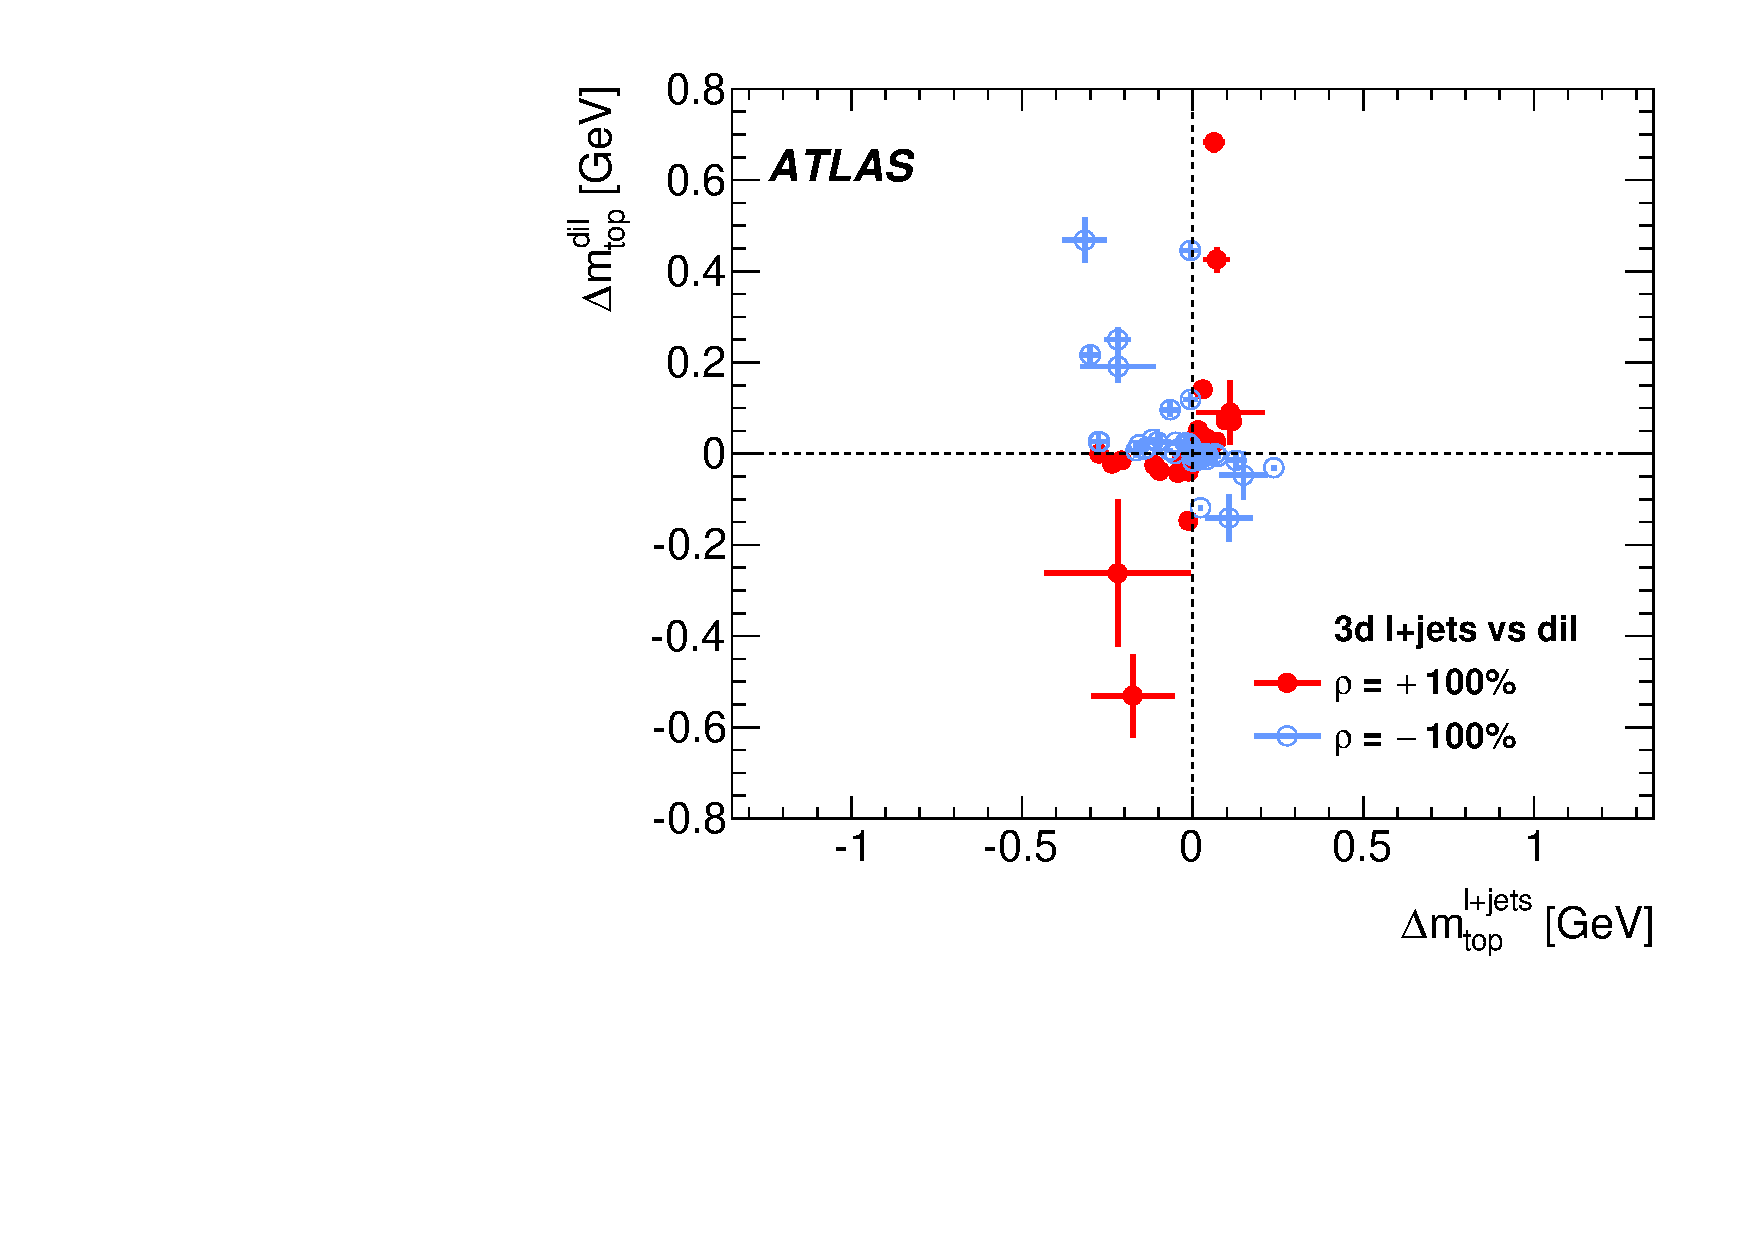
\includegraphics[width=0.33\textwidth]{./figs/SystCorr_TG_LJDL_fit3d1.pdf}
  \label{sfig:corrll3dlj}
}
\subfloat[2d \ljets\ ]{
  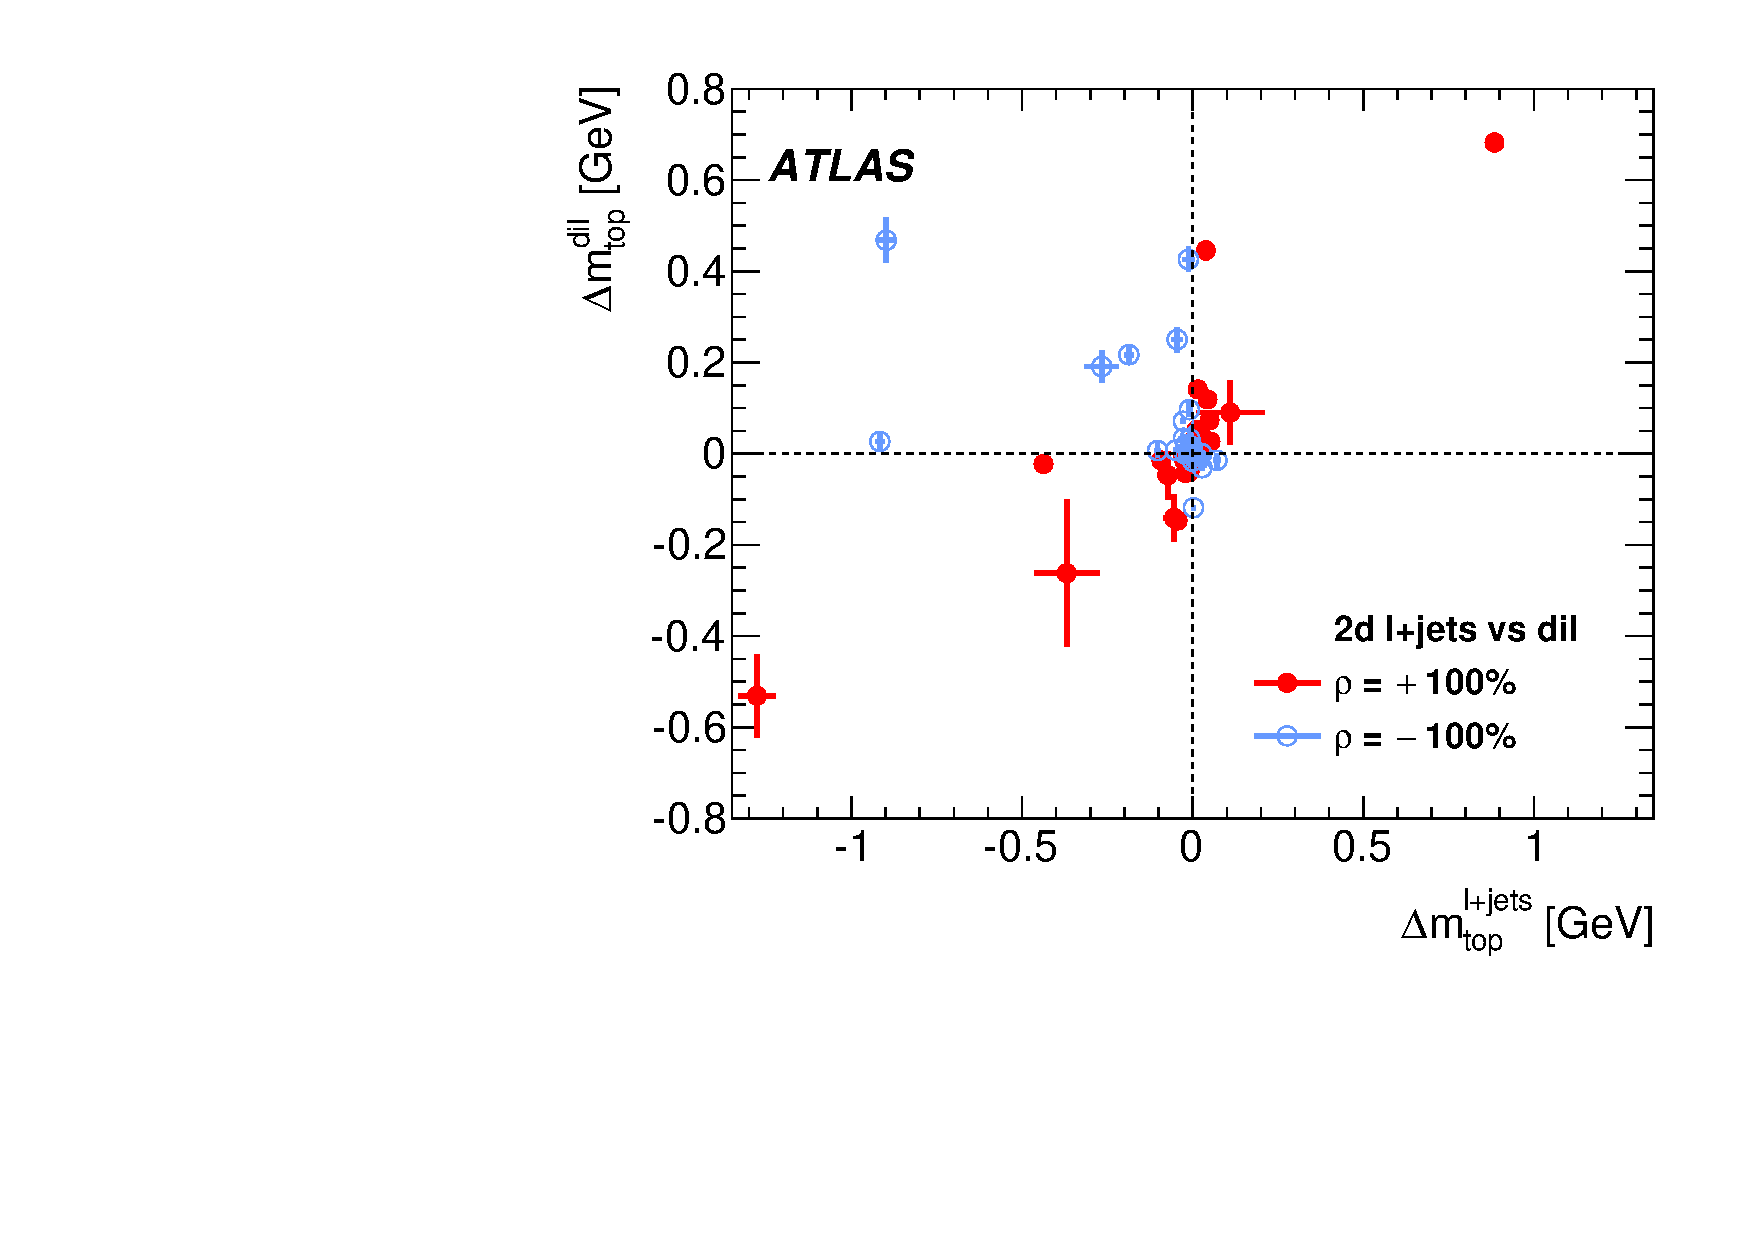
\includegraphics[width=0.33\textwidth]{./figs/SystCorr_TG_LJDL_fit3d0.pdf}
  \label{sfig:corrll2dlj}
}
\subfloat[1d \ljets\ ]{
  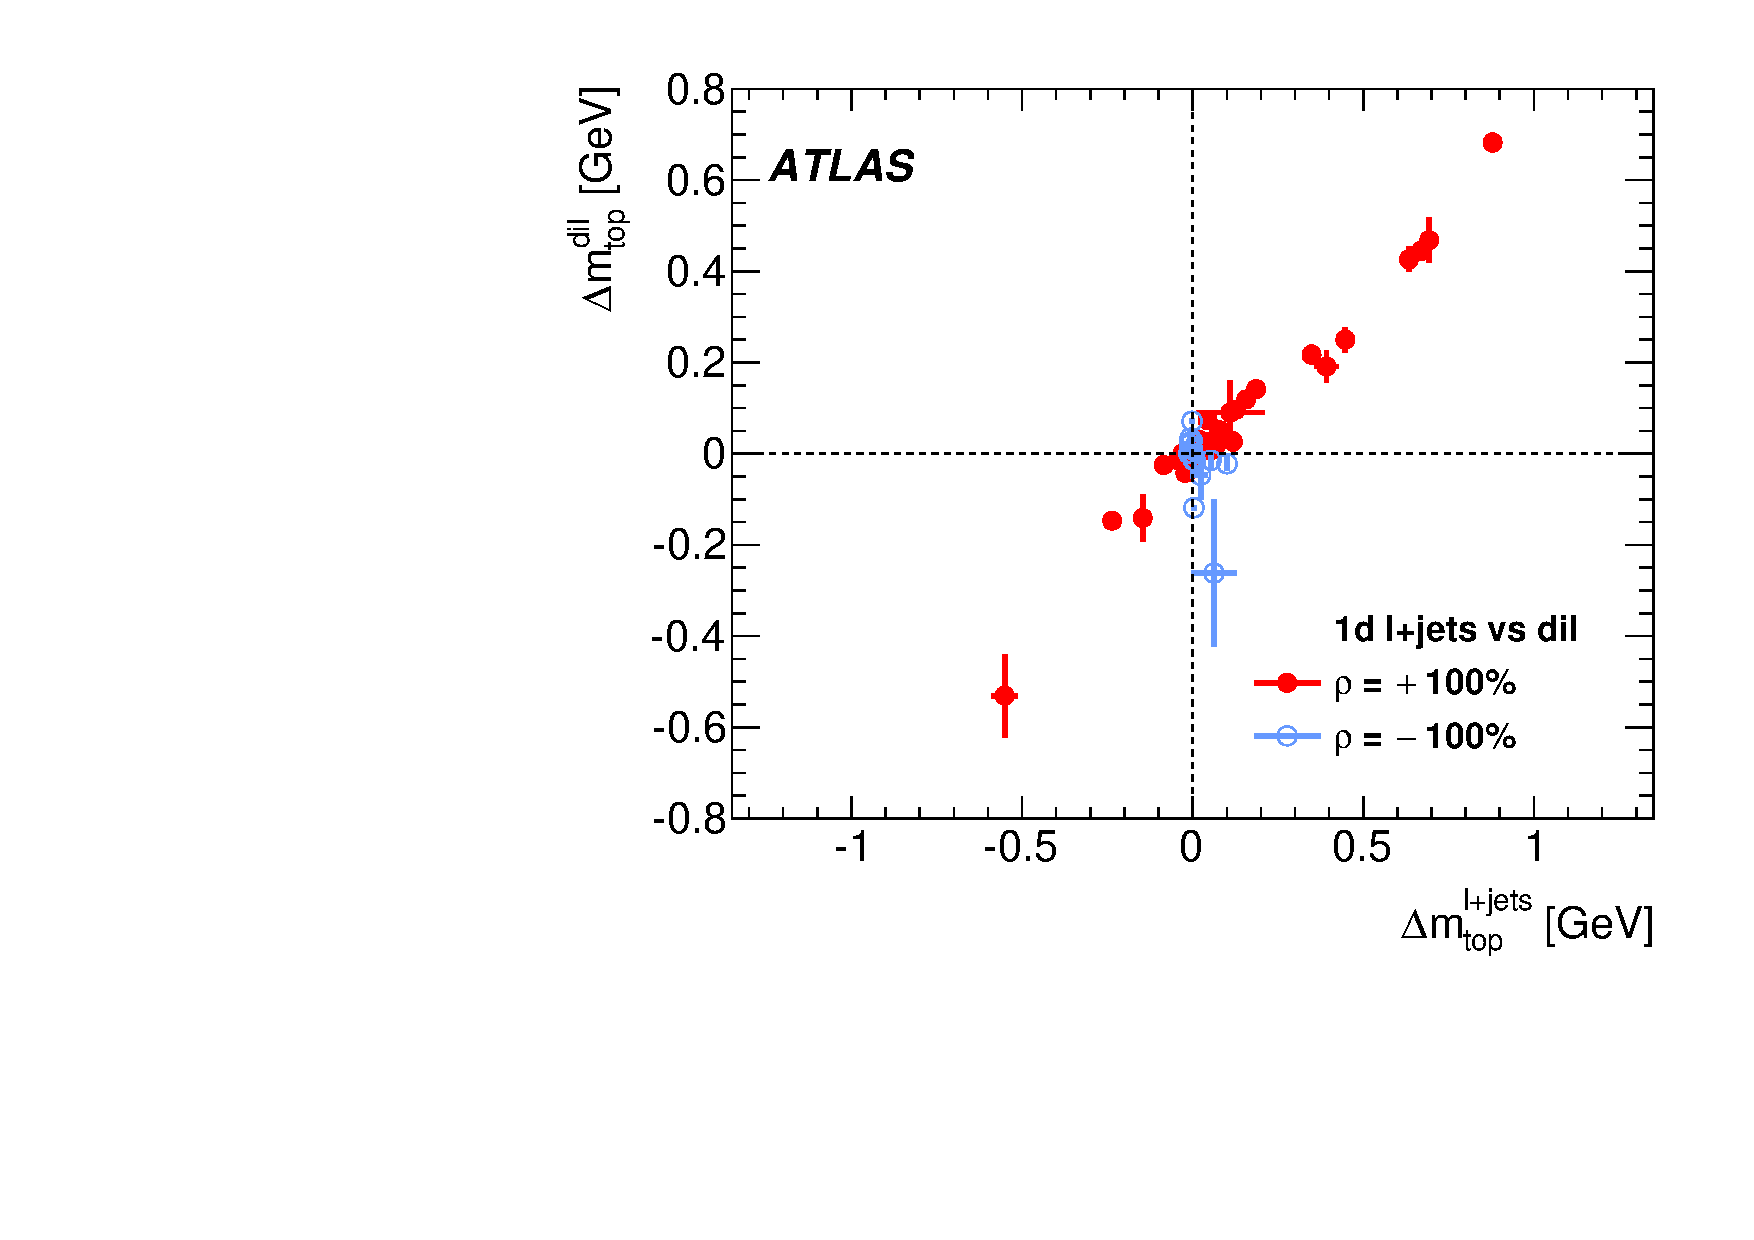
\includegraphics[width=0.33\textwidth]{./figs/SystCorr_TG_LJDL_fit3d-1.pdf}
  \label{sfig:corrll1dlj}
}
% \hfill
% \subfloat[3d \ljets\ ]{
%   \includegraphics[width=0.33\textwidth]{./figs/bjes_LJDL_systcorr_103.pdf}
%   \label{sfig:corrllbjes3dlj}
% }
% \subfloat[2d \ljets\ ]{
%   \includegraphics[width=0.33\textwidth]{./figs/bjes_LJDL_systcorr_102.pdf}
%   \label{sfig:corrllbjes2dlj}
% }
% \subfloat[1d \ljets\ ]{
%   \includegraphics[width=0.33\textwidth]{./figs/bjes_LJDL_systcorr_101.pdf}
%   \label{sfig:corrllbjes1dlj}
% }
\caption[Estimator correlations for the $\sqrts=7$~\TeV\ analyses]{
%
The systematic uncertainties of \mt\ in the \dil\ analysis versus those of the \subref{sfig:corrll3dlj} \threed, \subref{sfig:corrll2dlj} \twod and \subref{sfig:corrll1dlj} \oned \ljets\ analysis.
%
Sources for which the two estimators are fully \mbox{(anti-)}correlated are shown in red (blue).
%
% \Fig{s}~\subref{sfig:corrllbjes3dlj}, \subref{sfig:corrllbjes2dlj} and \subref{sfig:corrllbjes1dlj} show results of 500 pseudo-experiments for the \gls{bJES} uncertainty, with the up (red) and down (blue) variation, for the \dil\ analysis versus the \ljets\ analysis with different dimensionality. 
%
The points show the estimated systematic uncertainties on \mt\ for the two analyses and the uncertainty crosses reflect the corresponding statistical uncertainties. }
%
\label{fig:LJDLsystCorrTG7TeV}
%
\end{figure*}
%%%%%%%%%%%%%%%%%%%%%%%%%%%%%%%%%%%%%%%%%%%%%%%%%%%%%%%%%%%%%%%%%%%%%%%%%%%%%%%
%
%
The effect of the additional dimensions in the \ljets\ analysis is twofold: a reduction of single measurement uncertainties and a decorrelation effect, thus improving the gain of a combination. 
%
This can be seen in \fig~\ref{fig:LJDLsystCorrTG7TeV}. For an unchanged \dil\ analysis, the analysis in the \ljets\ channel has been performed with three dimensions~\subref{sfig:corrll3dlj}, with two dimensions~\subref{sfig:corrll2dlj}, fixing the \gls{bJSF} to unity, and with one dimension~\subref{sfig:corrll1dlj}, fixing in addition the \gls{JSF} to unity, only leaving \mt\ free in the fit. 
%
The figures show that the dominant uncertainties, which have the greatest distance to $\dmtlj=0$~\GeV\ in \fig~\subref{sfig:corrll1dlj}, are shifted towards the center, as a consequence of higher dimensionality and the corresponding higher constraining power. 
%
Most striking is the case of the \gls{bJES} uncertainty, which changes from the dominant right-most position in \fig~\subref{sfig:corrll2dlj} to an almost negligible size in \fig~\subref{sfig:corrll3dlj} due to the discriminative power of the \rbqr estimator. 
%
% \Fig{s}~\subref{sfig:corrllbjes3dlj} to \subref{sfig:corrllbjes1dlj} show the pseudo-experiments performed for the \gls{bJES} uncertainty as showcase. Also here, the drastic reduction in uncertainty is visible. 
%
Additionally, the almost diagonal alignment of the \mt\ shifts in \fig~\subref{sfig:corrll1dlj} shows the large similarity and correlation of the two \oned\ estimators, while the decorrelating effect of additional dimensions is visible from \fig~\subref{sfig:corrll2dlj} to \subref{sfig:corrll3dlj}. 


The guideline of minimising the correlation of the \ljets\ and \dil\ channels has been followed and has lead to the decision to not propagate the \gls{JSF} and \gls{bJSF} factors, measured in the \ljets\ analysis to the \dil\ analysis. 
%
Not only would the knowledge of \mt\ not increase that way and the combination result not improve~\cite{Aaltonen2009}, but secondly, a scale transfer would require an additional systematic uncertainty to account for the differences in kinematic selection and jet topologies of the two channels. 














\subsection{The combination}
\label{sec:7TeVcombination}
%
The results obtained for the \ttbarll\ and \ttbarlj\ channels, which are listed in \tab~\ref{tab:llandljresults7TeV}, are combined using the \gls{BLUE} method. 
%
The two measurements are compatible at the level of $0.75$ standard deviations, corresponding to a mass difference of $\mtlj-\mtdl = -1.47 \pm 1.96~\GeV$. 
%
The combination of the results yields:
%
\[
\mtcb = \XZ{172.99}{0.48}{0.78}~\GeV = \XZtot{172.99}{0.91}~\GeV
\]
%
This corresponds to a $28\%$ gain in precision with respect to the more precise single measurement, which is the measurement in the \ttbarlj\ channel. 
%
The total correlation of the two measurements is $-0.07$ and the $\chi^2$ probability of the combination is $45.5\%$. 
%
The \gls{BLUE} weights of the \ttbarll\ and \ttbarlj\ analyses are +0.452 and +0.548, respectively.
%
%
%%%%%%%%%%%%%%%%%%%%%%%%%%%%%%%%%%%%%%%%%%%%%%%%%%%%%%%%%%%%%%%%%%%%%%%%%%%%%%%
\begin{figure*}[tbp!]
\centering
\subfloat[Combined central value]{
  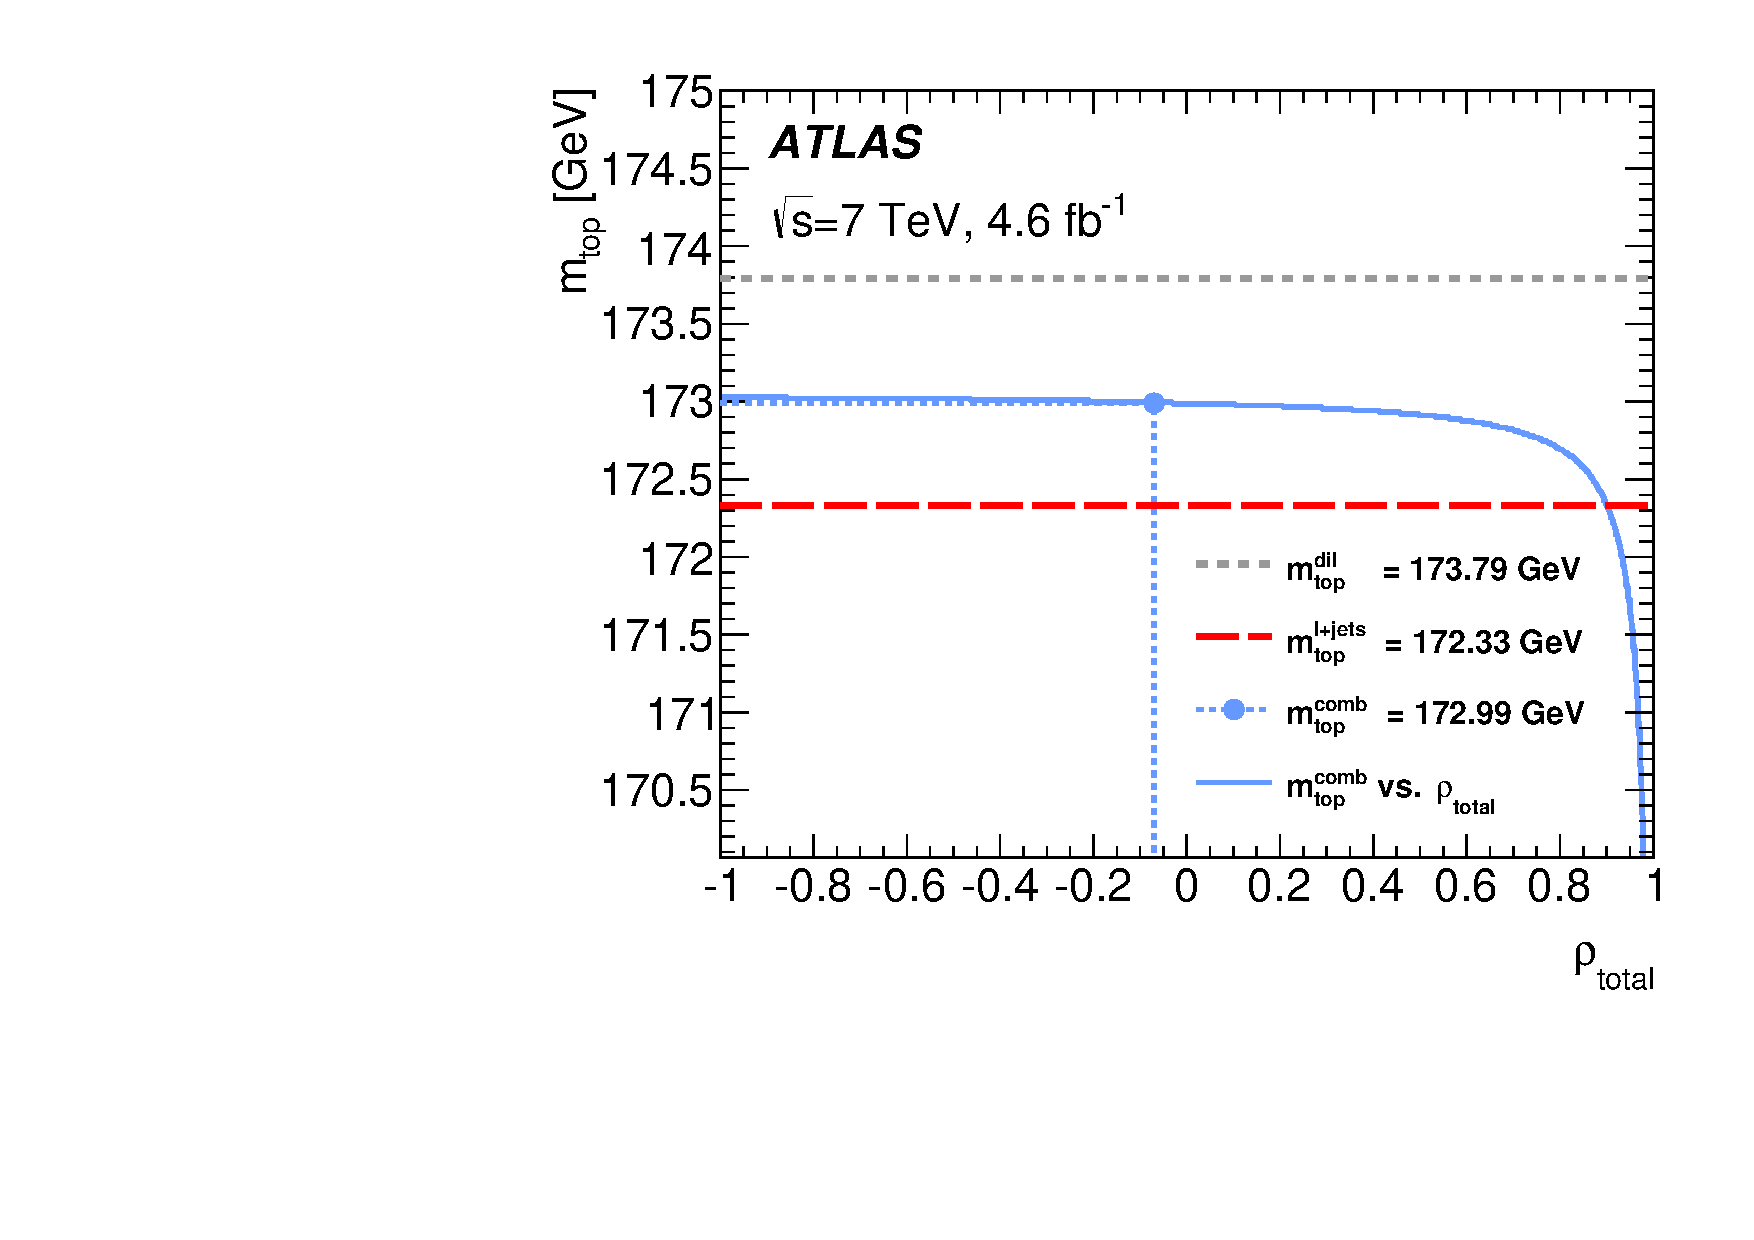
\includegraphics[width=0.49\textwidth]{./figs/CombValRhoDep.pdf}
  \label{sfig:CombValRhoDep}
}
\subfloat[Combined total uncertainty]{
  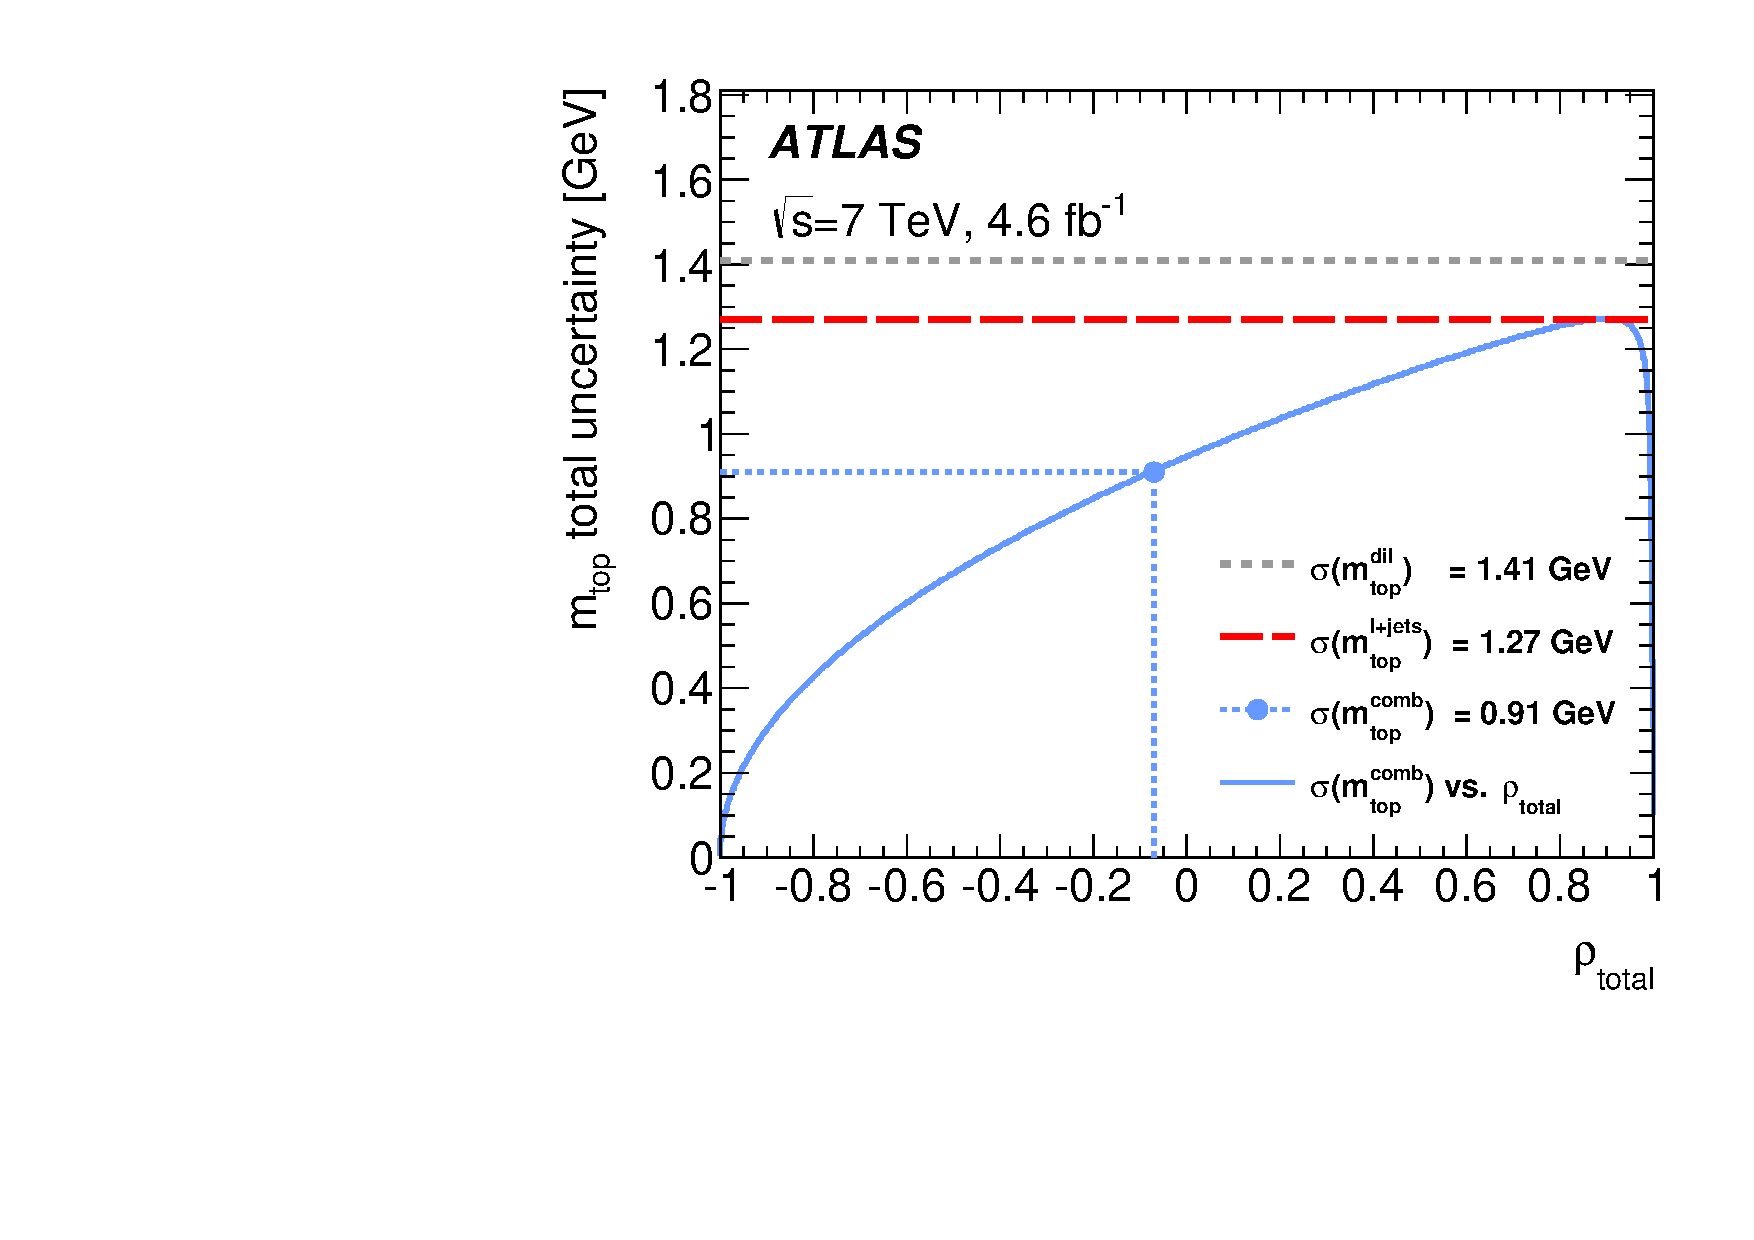
\includegraphics[width=0.49\textwidth]{./figs/CombUncRhoDep.pdf}
  \label{sfig:CombUncRhoDep}
}
\hfill
\caption[Stability of the combination for $\sqrts=7$~\TeV\ data]{
%
The dependence of the central value~\subref{sfig:CombValRhoDep} and the final uncertainty~\subref{sfig:CombUncRhoDep} of the combined result (blue) of the \gls{ATLAS} combination at $\sqrts=7~\TeV$~\cite{Aad:2015nba} as a function of the total correlation. For comparison, the corresponding values for the input measurements are also shown (grey and red dashed lines).
  \label{fig:combinationrho}}
\end{figure*}
%%%%%%%%%%%%%%%%%%%%%%%%%%%%%%%%%%%%%%%%%%%%%%%%%%%%%%%%%%%%%%%%%%%%%%%%%%%%%%%





\subsection{Stability of the results}
\label{sec:stabtests}
%
The input uncertainties to the \gls{BLUE} combination are subject to statistical fluctuations of the systematic uncertainties. Therefore, the stability of the combination results has been investigated by performing 1000 \gls{BLUE} combinations, in which the uncertainties are randomly varied according to a Gaussian \gls{pdf} with a width corresponding to their statistical uncertainty. 
%
In the process, the correlation assignments are reevaluated as well. 
%
The resulting combination values are Gaussian distributed with a width of 37~\MeV\ for the central value and 43~\MeV\ for the total uncertainty. 
%
The \gls{BLUE} combination weights and the total correlation values are similarly Gaussian distributed, with widths of $0.025$ and $0.06$, respectively.
%
These effects are negligible, compared to the total uncertainty of the combined result and no additional systematic uncertainty is assigned. 
%
The dependence of the central value and the total uncertainty on the total correlation is displayed in \fig~\ref{fig:combinationrho}. The uncertainty on the determined correlation of $2.5\%$ is small compared to the axis scale and corresponds to an insignificant change of the results. This shows the stability of the estimate. 







\subsection{Comparison to the traditional correlation scenario}
%
The combination presented here relies on a direct evaluation of the correlations of uncertainty sources. A comparison with the traditional correlation scenario discussed in \sect~\ref{sect:prevcomb} is given in \tab~\ref{tab:corrcomp}, showing the correlations, which have been assigned as either $+100\%$ or $0\%$ based on the physics arguments in the \gls{LHC} combination~\cite{LHC2013}, and the evaluated ones from \tab~\ref{tab:llandljresults7TeV}. Based on the same input except for the correlations, the combination has been reperformed and the resulting combined uncertainty components for the leading uncertainty sources are given.
%
This shows that the 22\% precision gain with respect to the traditional correlation scenario is a consequence of the exploitation of anti-correlations, which may lead to a significant reduction or even complete cancellation of the combined uncertainty, such as the \gls{ISRFSR} and the \gls{JER} uncertainties. The dominant \gls{JES} uncertainty is also significantly reduced.
%
This shows the potential precision gain from a determination instead of an assignment of correlations.
%
% -------------------------------------------------------
\begin{table*}[tbp!]
% \footnotesize
\begin{center}
\begin{tabular}{|l|c|c|c|c|}
\cline{2-5}
  \multicolumn{1}{c}{}
& \multicolumn{ 2}{|c|}{Assigned}
& \multicolumn{ 2}{c|}{Evaluated} \\
\hline
Uncertainty categories & $\rho$ &  $\mtcb$ [\GeV]&  $\rho$  & $\mtcb$ [\GeV]\\
\hline
Result                                 & $    $ & $172.91$ & $     $ & $172.99$ \\
% Statistics                           & $ 0.00$ & $  0.50$ & $ 0.00$ & $  0.48$ \\
% Method                               & $ 0.00$ & $  0.08$ & $ 0.00$ & $  0.07$ \\
% Signal \glsdesc{MC} generator        & $+1.00$ & $  0.24$ & $+1.00$ & $  0.24$ \\
Hadronisation                          & $+1.00$ & $  0.32$ & $+1.00$ & $  0.34$ \\
\glsdesc{ISRFSR}                       & $+1.00$ & $  0.38$ & $-1.00$ & $  0.04$ \\
% \glsdesc{UE}                         & $+1.00$ & $  0.11$ & $-1.00$ & $  0.06$ \\
\glsdesc{CR}                           & $+1.00$ & $  0.12$ & $-1.00$ & $  0.00$ \\
% \glsdesc{PDF}                        & $+1.00$ & $  0.19$ & $+0.57$ & $  0.17$ \\
% $W/Z$+jets normalisation             & $+1.00$ & $  0.02$ & $+1.00$ & $  0.02$ \\
% $W/Z$+jets shape                     & $+1.00$ & $  0.17$ & $ 0.00$ & $  0.16$ \\
% \fake normalisation                  & $ 0.00$ & $  0.06$ & $+1.00$ & $  0.07$ \\
% \fake shape                          & $ 0.00$ & $  0.03$ & $+0.23$ & $  0.03$ \\
\glsdesc{JES}                          & $+1.00$ & $  0.65$ & $-0.23$ & $  0.41$ \\
\glsdesc{bJES}                         & $+1.00$ & $  0.31$ & $+1.00$ & $  0.34$ \\
\glsdesc{JER}                          & $+1.00$ & $  0.21$ & $-1.00$ & $  0.03$ \\
% \glsdesc{JRE}                        & $+1.00$ & $  0.10$ & $+1.00$ & $  0.10$ \\
% \glsdesc{JVF}                        & $+1.00$ & $  0.01$ & $-1.00$ & $  0.01$ \\
\btag                                  & $+1.00$ & $  0.33$ & $-0.77$ & $  0.25$ \\
% Leptons                              & $+1.00$ & $  0.08$ & $-0.34$ & $  0.06$ \\
% \met                                 & $+1.00$ & $  0.11$ & $-0.15$ & $  0.08$ \\
% Pile-up                              & $+1.00$ & $  0.02$ & $ 0.00$ & $  0.01$ \\
\hline
Total Syst                             & $     $ &  $1.05$ & $     $ & $0.78$ \\
Total                                  & $+0.51$ &  $1.16$ & $-0.07$ & $0.91$ \\
\hline
Relative precision gain                &   \multicolumn{ 2}{c|}{$9\%$}  &  \multicolumn{ 2}{c|}{$28\%$}  \\
% \hline
% % Source                 & \begin{turn}{90}LHC comb.\end{turn} & \begin{turn}{90}BLUE\end{turn} & \begin{turn}{90}ATLAS comb.\end{turn}  & \begin{turn}{90}ATLAS comb.\end{turn} \\
% Values taken from      & [2] &  BLUE & \multicolumn{ 2}{c|}{[1]} \\
\hline
\end{tabular}
\end{center}
\caption[Comparison of correlation scenarios]{
%
Comparison of the traditional correlation scenario with assignments of $+100\%$ or $0\%$ correlation based on physics arguments with the results of the direct correlation evaluation. 
%
For a selection of uncertainty sources, the assigned or evaluated correlations are shown together with the resulting uncertainties of the standard scenario. The relative precision gain with respect to the most precise input measurement is given as well.
%
Uncertainty sources either leading in size or with significant gain in precision are shown.
%
\label{tab:corrcomp}}
\end{table*}
% -------------------------------------------------------
%
%























\section[Combination of the \texorpdfstring{$\sqrts=7$}{sqrt(s)=7} and 8~\TeV\ measurements]{Combination of the \texorpdfstring{\boldmath$\sqrts=7$ and \boldmath$8~\TeV$}{sqrt(s)=7 and 8~\TeV} measurements}
\label{sec:resultcomb78TeV}
%
The combination of the \ttbarlj\ and \ttbarll\ results at $\sqrts=7$~\TeV\ with the \ttbarll\ result at $\sqrts=8$~\TeV\ from the \mvabased\ analysis is described in this section. 
%
All quantities related to the central values of the $\sqrts=8$~\TeV\ analyses are subject to the constant but unknown blinding shift, described in \sect~\ref{sect:application8TeV}. Therefore, compatibility studies of different \cmes\ are performed for completeness, but carry limited information. An up and down variation of the blinded central value at $\sqrts=8$~\TeV\ by this shift is performed to obtain an estimate of its impact on the combination.
%
The evaluation of the correlations, introduced for the $\sqrts=7$~\TeV\ combination, has been used. While the treatment of uncertainty categories for the two measurements at $\sqrts=7$~\TeV\ follows the approach outlined in the previous section, for a combination with the results at $\sqrts=8$~\TeV\ a mapping of uncertainty categories for data taken at different \cmes\ has to be set up. 
%
Non-trivial cases are the uncertainty components involving eigenvector decompositions like the \gls{JES} and \btag\ scale uncertainties, or uncertainty categories that have been added or removed. 
%
For the \gls{JES}, two scenarios have been proposed for a combined treatment, a weak and a strong correlation scenario~\cite{JEScorrelationScenarios}. The two scenarios relate the \glspl{NuP} of the different \gls{JES} categories to the ones at $\sqrts=7$~\TeV, as shown in \tab~\ref{tab:jesresults8TeV}. Components without an equivalent at the other \cme\ are treated as independent. The strong correlation scenario assumes full correlation for several uncertainty components resulting from eigenvector decomposition, e.g. the modelling uncertainties, while the weak correlation scenario only relates the components where an unambiguous equivalent can be identified. Since the true correlation is unknown, the weak correlation scenario is taken as default and the strong correlation setup serves as stability check.
%
The $\sqrts=7$ and $8$~\TeV\ measurements are treated as uncorrelated for the \glspl{NuP} of the $b$-, $c$-, $\tau$- and mistagging uncertainties. A correlated treatment of the flavour tagging \glspl{NuP} yields no difference in the combination.
%% https://twiki.cern.ch/twiki/bin/viewauth/AtlasProtected/JESCorrelationRecommendations
%
%--------------------------------------------------------------------------
\begin{table*}[thp!]
% \footnotesize
%\small
\begin{center}
\begin{tabular}{|l|r|l|}\cline{2-3}
%%%%%%%%%%%%%%%%%%%%%%%%%%%%%%%%%%%%%%%%%%
%%%%%%% VALUES FOR CUTBASED DILEPTON  %%%%
%%%%%%%%%%%%%%%%%%%%%%%%%%%%%%%%%%%%%%%%%%
% 0.13 \pm 0.00 
% +0.03 \pm 0.01
% +0.01 \pm 0.00
% -0.07 \pm 0.00
% +0.07 \pm 0.01
% +0.08 \pm 0.01
%  0.37 \pm 0.00
% +0.35 \pm 0.02
% +0.02 \pm 0.09
% -0.05 \pm 0.01
% +0.03 \pm 0.00
% +0.08 \pm 0.01
%  0.25 \pm 0.00
% +0.25 \pm 0.01
% -0.01 \pm 0.01
% +0.02 \pm 0.00
%  0.19 \pm 0.00
% +0.18 \pm 0.01
% -0.02 \pm 0.01
% -0.06 \pm 0.00
% +0.01 \pm 0.00
%  0.00 \pm 0.00
%  0.22 \pm 0.00
% -0.01 \pm 0.00
% -0.02 \pm 0.00
% +0.02 \pm 0.00
% +0.22 \pm 0.00
% +0.01 \pm 0.00
%  0.02 \pm 0.00
% +0.00 \pm 0.00
% -0.02 \pm 0.00
% +0.31 \pm 0.01
%  0.55 \pm 0.01
%%%%%%%%%%%%%%%%%%%%%%%%%%%%%%%%%%%%%%%%%%
\multicolumn{1}{c|}{}                            &     $\Delta\mt$ [\GeV]   & \multicolumn{1}{c|}{Mapping to $\sqrts=7$~\TeV}          \\ \hline
\textbf{Statistical (total)}                     &\boldmath$0.14 \pm 0.02 $ & \multicolumn{1}{c|}{--}                          \\
$~~~$ Statistical \gls{NuP}1                     &         $+0.04 \pm 0.01$ & \multicolumn{1}{c|}{--}                          \\         
$~~~$ Statistical \gls{NuP}2                     &         $+0.01 \pm 0.00$ & \multicolumn{1}{c|}{--}                          \\         
$~~~$ Statistical \gls{NuP}3                     &         $-0.07 \pm 0.01$ & \multicolumn{1}{c|}{--}                          \\
$~~~$ Statistical \gls{NuP}4                     &         $+0.06 \pm 0.01$ & \multicolumn{1}{c|}{--}                          \\
$~~~$ $\eta$ inter-calibration (stat.)           &         $+0.09 \pm 0.01$ & \multicolumn{1}{c|}{--}                          \\
\textbf{Modelling (total)}                       &\boldmath$ 0.33 \pm 0.01$ & \multicolumn{1}{c|}{--}                          \\
$~~~$ Modelling \gls{NuP}1                       &         $+0.31 \pm 0.01$ & Modelling \gls{NuP}1 {\bf \color{red}(strong)}   \\        
$~~~$ Modelling \gls{NuP}2                       &         $+0.01 \pm 0.00$ & Modelling \gls{NuP}2 {\bf \color{red}(strong)}   \\         
$~~~$ Modelling \gls{NuP}3                       &         $-0.06 \pm 0.00$ & Modelling \gls{NuP}3 {\bf \color{red}(strong)}   \\         
$~~~$ Modelling \gls{NuP}4                       &         $+0.04 \pm 0.00$ & Modelling \gls{NuP}4 {\bf \color{red}(strong)}   \\
$~~~$ $\eta$ inter-calibration (model)           &         $+0.09 \pm 0.01$ & $\eta$ inter-calib. (model)                      \\
\textbf{Detector (total)}                        &\boldmath$ 0.19 \pm 0.01$ & \multicolumn{1}{c|}{--}                          \\
$~~~$ Detector \gls{NuP}1                        &         $+0.19 \pm 0.01$ & Detector \gls{NuP}1                              \\         
$~~~$ Detector \gls{NuP}2                        &         $+0.00 \pm 0.00$ & \multicolumn{1}{c|}{--}                          \\
$~~~$ Detector \gls{NuP}3                        &         $+0.02 \pm 0.00$ & Detector \gls{NuP}2 {\bf \color{red}(strong)}    \\
\textbf{Mixed (total)}                           &\boldmath$ 0.16 \pm 0.01$ & \multicolumn{1}{c|}{--}                          \\
$~~~$ Mixed \gls{NuP}1                           &         $+0.15 \pm 0.01$ & Mixed \gls{NuP}1 {\bf \color{red}(strong)}       \\         
$~~~$ Mixed \gls{NuP}2                           &         $-0.03 \pm 0.01$ & \multicolumn{1}{c|}{--}                          \\
$~~~$ Mixed \gls{NuP}3                           &         $-0.05 \pm 0.00$ & \multicolumn{1}{c|}{--}                          \\
$~~~$ Mixed \gls{NuP}4                           &         $+0.01 \pm 0.00$ & Mixed \gls{NuP}2 {\bf \color{red}(strong)}       \\
\textbf{Single particle high-\boldmath$\pt$}     &\boldmath$ 0.00 \pm 0.00$ & Single part. high-\pt                            \\
\textbf{Pile-up (total)}                         &\boldmath$ 0.20 \pm 0.00$ & \multicolumn{1}{c|}{--}                          \\
$~~~$ Pile-up: offset ($\mu$)                    &         $-0.01 \pm 0.00$ & Pile-up: offset ($\mu$)                          \\         
$~~~$ Pile-up: offset ($n_{\rm vtx}$)            &         $-0.04 \pm 0.00$ & Pile-up: offset ($n_{\rm vtx}$)                  \\ 
$~~~$ Pile-up: \pt                               &         $+0.03 \pm 0.00$ & \multicolumn{1}{c|}{--}                          \\ 
$~~~$ Pile-up: $\rho$                            &         $+0.20 \pm 0.00$ & \multicolumn{1}{c|}{--}                          \\ 
\textbf{Punch-through}                           &\boldmath$+0.01 \pm 0.00$ & \multicolumn{1}{c|}{--}                          \\
\textbf{Flavour (total)}                         &\boldmath$ 0.00 \pm 0.00$ & \multicolumn{1}{c|}{--}                          \\
$~~~$ Flavour composition                        &         $ 0.00 \pm 0.00$ & Flavour composition                              \\         
$~~~$ Flavour response                           &         $ 0.00 \pm 0.00$ & Flavour response                                 \\
\textbf{\gls{bJES}}                              &\boldmath$+0.31 \pm 0.01$ & \gls{bJES}                                       \\ \hline %\cline{1-2}
   Total (without \gls{bJES})                    &         $ 0.48 \pm 0.00$ &                                                  \\ \hline
                                                 % &                          & \textbf{Relative non-closure \gls{MC}}           \\
                                                 % &                          & \textbf{Close-by jets}                           \\
\end{tabular}
\end{center}
\caption[\gls{JES} components for the $\sqrts=8$~\TeV\ analysis]{
%
The individual components of the \gls{JES} uncertainty observed in the $\sqrts=8$~\TeV\ analysis, together with the corresponding uncertainty on \mt~\cite{JESRecommendations2012Twiki}.
%
The main components are listed in bold-face and calculated as the sum in quadrature of the respective sub-components.
%
The weak and the strong correlation mapping to the uncertainty components at $\sqrts=7$~\TeV\ is also given~\cite{JEScorrelationScenarios}.
%
\label{tab:jesresults8TeV}}
\end{table*}
%--------------------------------------------------------------------------







The combination is performed with the \gls{BLUE} method, while individually treating all systematic subcomponents.
%
\Fig~\ref{fig:rhoeval78TeV} shows the observed \mt\ differences for the variation of all corresponding uncertainty subcomponents for the remaining pairs of the three measurements, as determined from pseudo-experiments for the $\sqrts=7$ and $8$~\TeV\ measurements, respectively. 
%
%Similar to \fig~\ref{fig:LJDLsystCorrTG7TeV}, the uncertainty components with a same sign effect on \mt\ are assigned a full correlation, while the ones with an opposite sign effect are assigned a full anti-correlation. 
%
Using these results, composite uncertainty sources are treated by adding the corresponding terms of the covariance matrices, resulting in a correlation different from $\pm 100\%$, as outlined in \sect~\ref{sec:sgncorr7TeV}. Besides the usual composite components based on eigenvector decomposition like the \gls{JES} uncertainty, this has also been applied to the background uncertainties corresponding to $\Wbos/\Zbos$ boson and \fake\ events. 

As expected, a positive correlation for the two measurements in the \dil\ channel is observed for most uncertainty components. 
%
An exception is the \gls{MC} generator uncertainty, i.e. the leftmost point in the upper left quadrant of \fig~\subref*{sfig:corr12}. Due to limited statistics in the \gls{MC} samples used for its evaluation, its size is not significantly different from zero and the assignment to a quadrant and the corresponding correlation is ambiguous. The impact of this on the combination results is evaluated using pseudo-experiments and found to be small.
%
The observed correlations of the $\sqrts=7$~\TeV\ \ljets\ and the $8$~\TeV\ \dil\ channel analyses are shown in \fig~\subref*{sfig:corr02}. The corresponding distribution for the two $\sqrts=7$~\TeV\ analyses has already been discussed in \sect~\ref{sec:sgncorr7TeV} and shown in \fig~\subref*{sfig:corrll3dlj}. In both figures, a similarly uncorrelated configuration is observed, due to the in-situ measurement of the \gls{JSF} and \gls{bJSF} in the \threed\ \ljets\ analysis.
%
%%%%%%%%%%%%%%%%%%%%%%%%%%%%%%%%%%%%%%%%%%%%%%%%%%%%%%%%%%%%%%%%%%%%%%%%%%%%%%%
\begin{figure*}[tbp!]
\centering
% \subfloat[Uncertainties of the $\sqrts=7$~\TeV\ analyses]{
% \subfloat[$\sqrts=7$~\TeV\ \dil\ vs \ljets]{
%   \includegraphics[width=0.49\textwidth]{./figs/fig_8TeV_TRC28_wp70_BDT-0.03/Combination_7_8TeV_correlation_12.pdf}
%   \label{sfig:corr01}
% }
% \subfloat[Uncertainties of the \dil\ analyses]{
\subfloat[$\sqrts=7$ vs $8$~\TeV\ \dil]{
  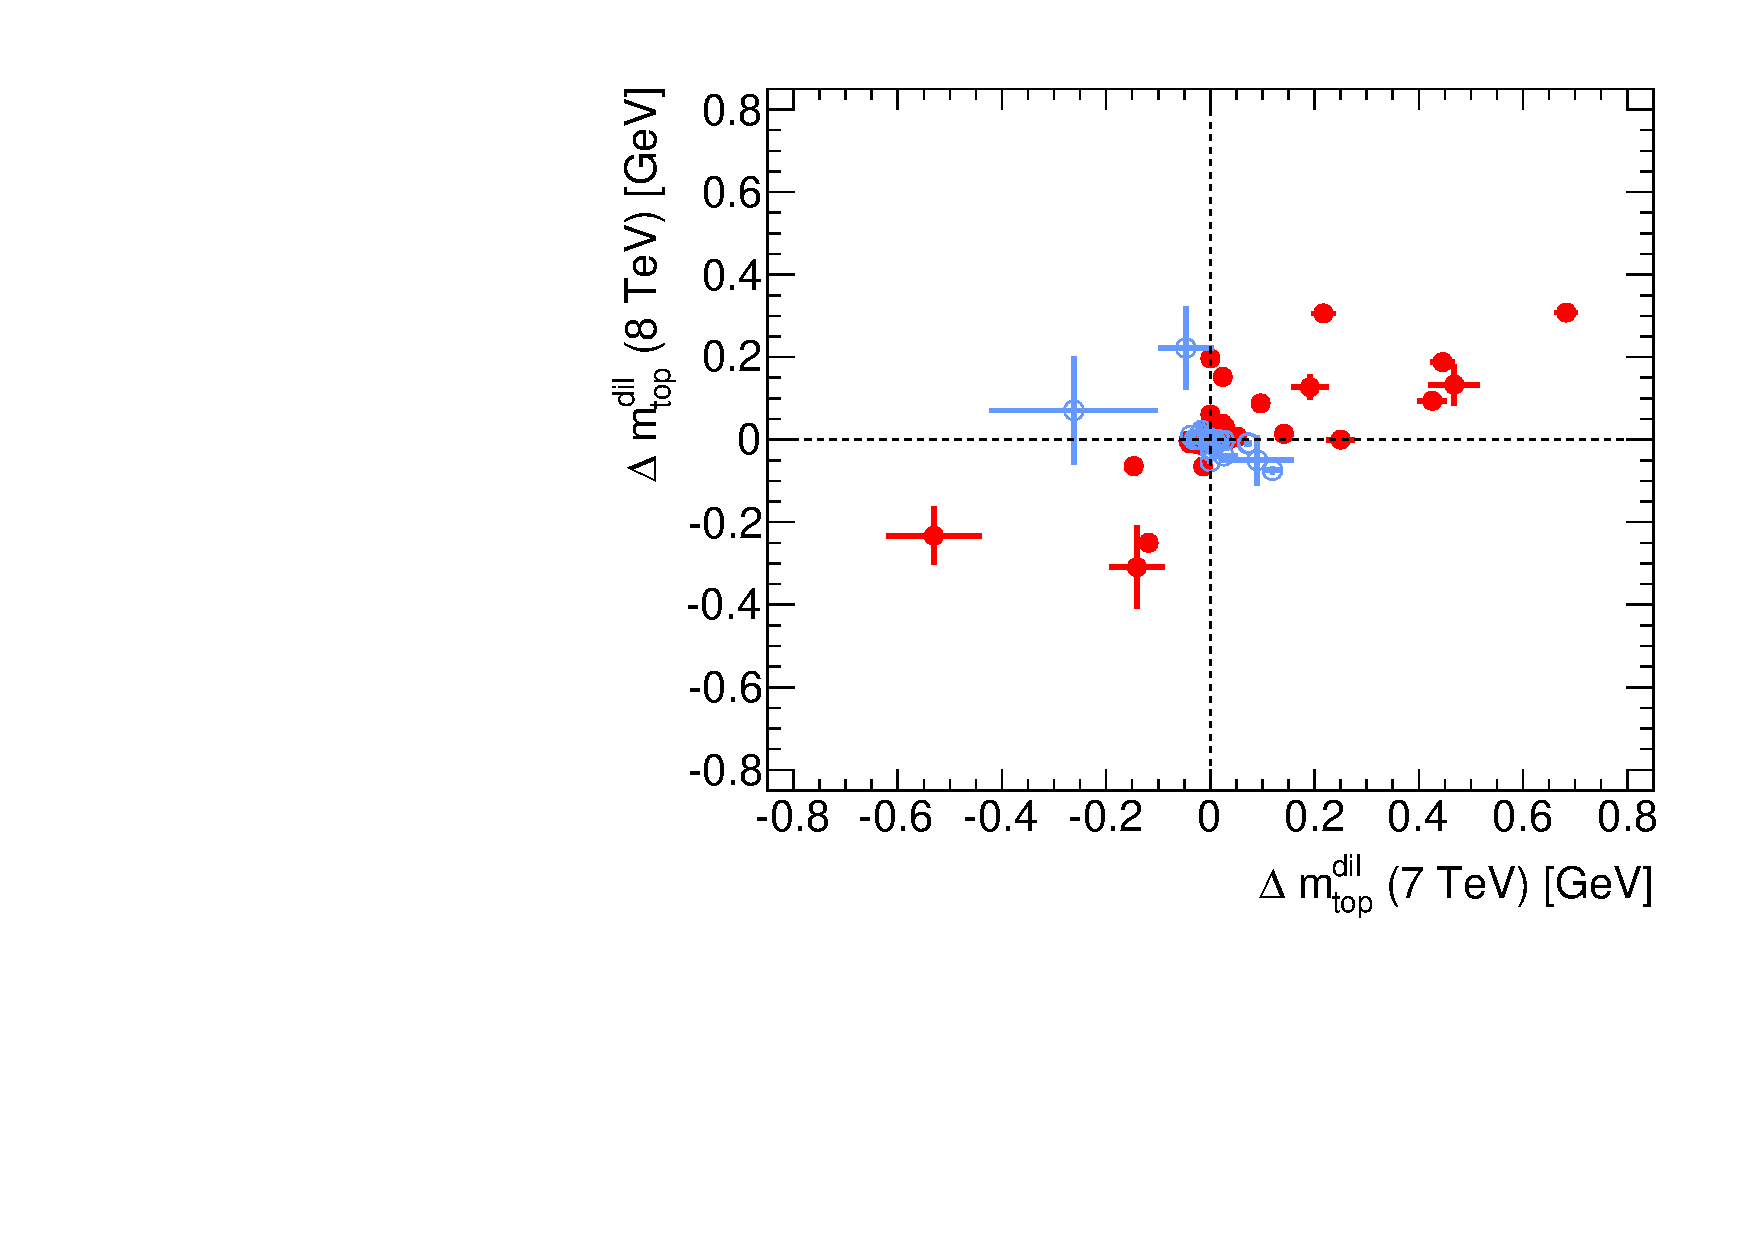
\includegraphics[width=0.49\textwidth]{./figs/fig_8TeV_TRC28_wp70/Combination_7_8TeV_correlation_01.pdf}
  \label{sfig:corr12}
}
\subfloat[$\sqrts=7$~\TeV\ \ljets\ vs  $\sqrts=8$~\TeV\ \dil]{
  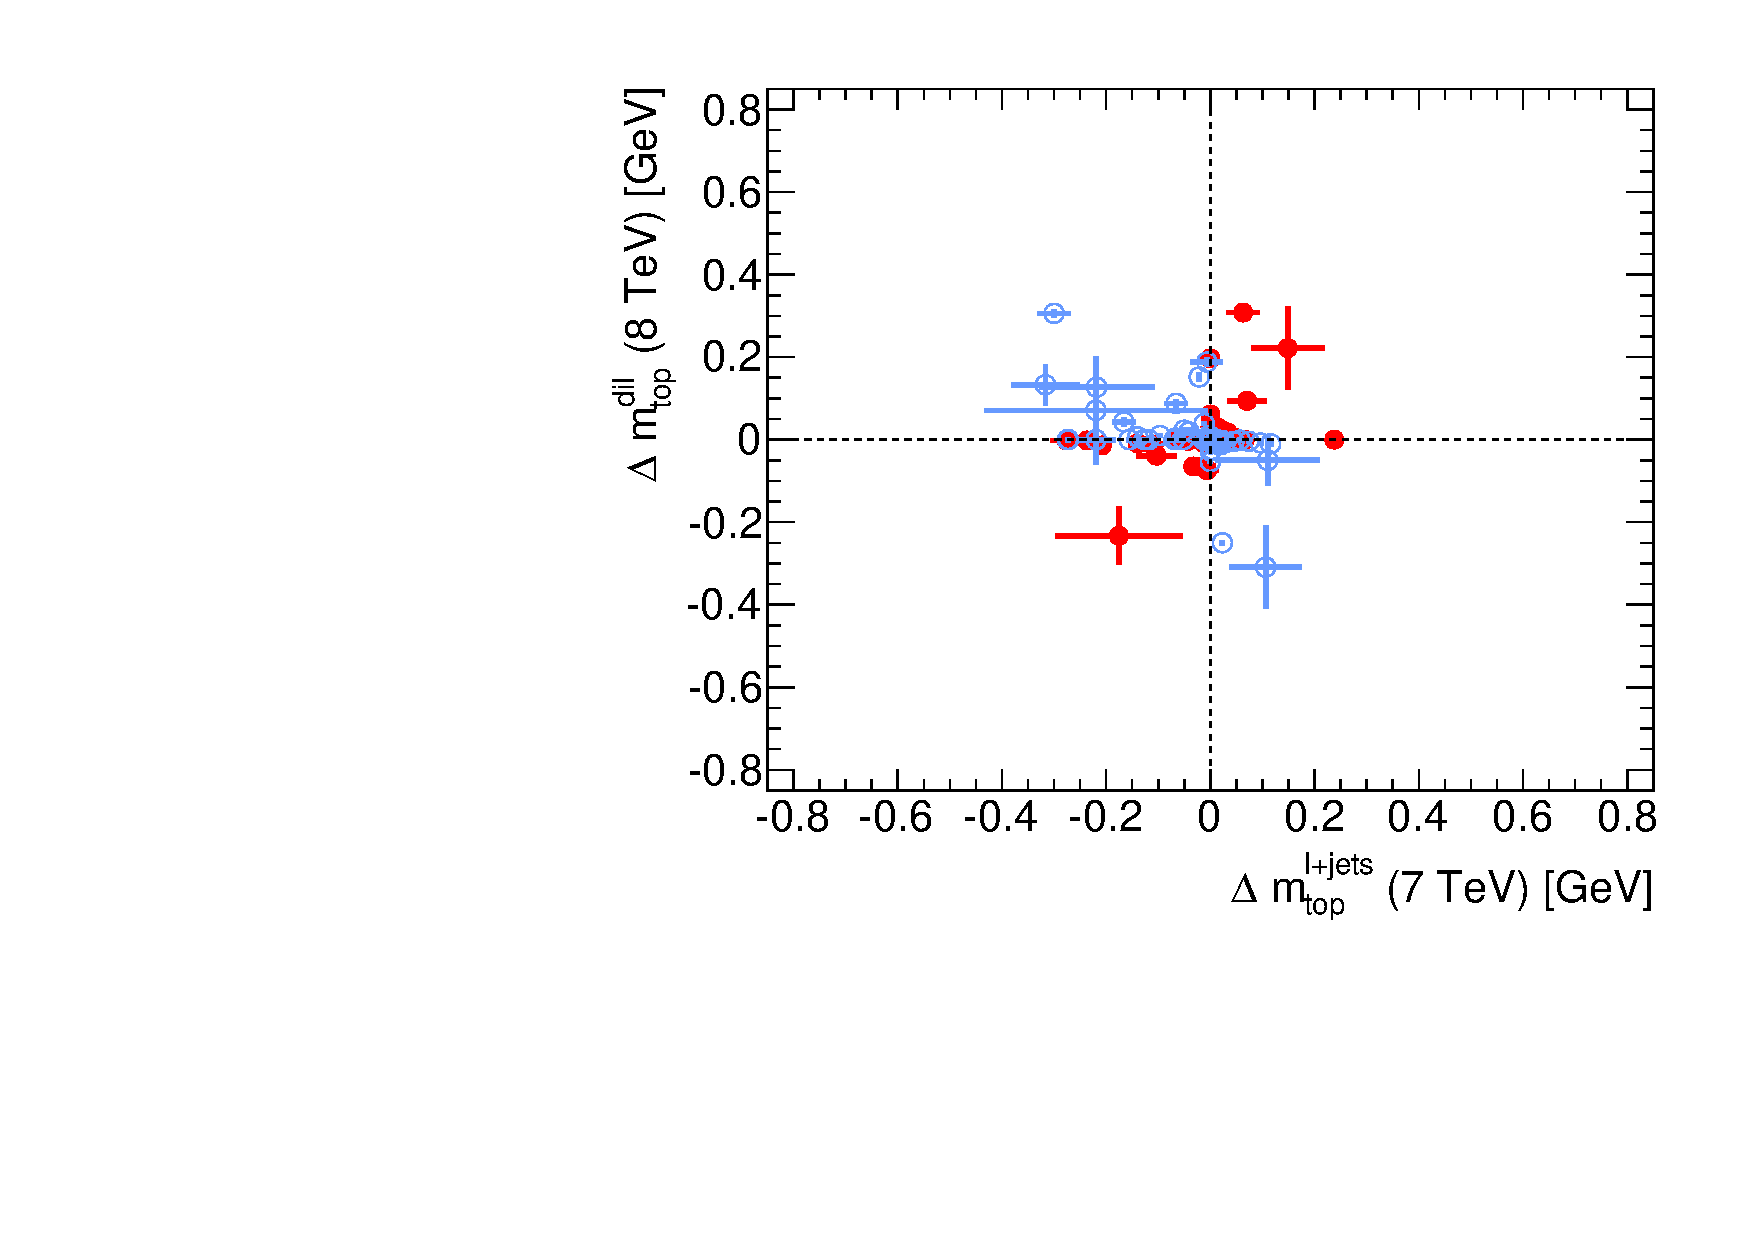
\includegraphics[width=0.49\textwidth]{./figs/fig_8TeV_TRC28_wp70/Combination_7_8TeV_correlation_02.pdf}
  \label{sfig:corr02}
}
% \hfill
\caption[Estimator correlations for the $\sqrts=7$ and $8$~\TeV\ analyses]{
%
%
The systematic uncertainties on \mt\ of the \dil\ analysis at $\sqrts=8$~\TeV\ versus those of the $\sqrts=7$~\TeV\ analyses. 
%
The uncertainty crosses indicate the statistical precision on the systematic uncertainty.
%
Sources for which the two estimators are fully (anti-)correlated are shown in red (blue).
%
\label{fig:rhoeval78TeV}}
\end{figure*}
%%%%%%%%%%%%%%%%%%%%%%%%%%%%%%%%%%%%%%%%%%%%%%%%%%%%%%%%%%%%%%%%%%%%%%%%%%%%%%%
%



The central values of the three measurements, their uncertainty components, the determined correlations of each pair of measurements and the results of the combinations are given in \tab~\ref{tab:resultscomb78TeV}.
%
%
%--------------------------------------------------------------------------
\begin{sidewaystable*}[tbp!]
%\footnotesize
\small
\begin{center}
\begin{tabular}{|l|r|r|r|r|r|r|r|r|r|} \cline{2-10}
\multicolumn{1}{c|}{}  	  & \multicolumn{2}{c|} {$\sqrts=7$~\TeV}    & $\sqrts=8$~\TeV       & \multicolumn{3}{c|} {Correlations}               &\multicolumn{3}{c|} {Combinations} \\ \cline{2-10}
\multicolumn{1}{c|}{}  	      &   \mtlj\ [\GeV]    &  \mtdl\ [\GeV]     &   \mtdl\ [\GeV]           & $\rho_{01} $ & $\rho_{02}$  & $\rho_{12}$ & \mtseven\ [\GeV] & \mtdl\ [\GeV] & \mtall\ [\GeV] \\ \hline
          Results             & 172.33             & 173.79             & \BDTValue                 & $     $      & $     $      & $     $     & 172.99    & \CombValueDL  & \CombValue    \\ \hline
       Statistics             &   0.75             &   0.54             & \BDTStat                  & $    0$      & $    0$      & $    0$     &   0.48    & \CombStatDL   & \CombStat     \\
            Method            &   0.11 $\pm$ 0.10  &   0.09 $\pm$ 0.07  &      0.05 $\pm$ 0.06      & $    0$      & $    0$      & $    0$     &   0.07    & 0.05          & 0.05          \\ \hline
Signal \glsdesc{MC} generator &   0.22 $\pm$ 0.21  &   0.26 $\pm$ 0.16  &      0.07 $\pm$ 0.13      & $+1.00$      & $-1.00$      & $-1.00$     &   0.24    & 0.04          & 0.05          \\
     Hadronisation            &   0.18 $\pm$ 0.12  &   0.53 $\pm$ 0.09  &      0.23 $\pm$ 0.07      & $+1.00$      & $+1.00$      & $+1.00$     &   0.34    & 0.26          & 0.24          \\
  \glsdesc{ISRFSR}            &   0.32 $\pm$ 0.06  &   0.47 $\pm$ 0.05  &      0.13 $\pm$ 0.05      & $-1.00$      & $-1.00$      & $+1.00$     &   0.04    & 0.16          & 0.02          \\
      \glsdesc{UE}            &   0.15 $\pm$ 0.07  &   0.05 $\pm$ 0.05  &      0.22 $\pm$ 0.10      & $-1.00$      & $+1.00$      & $-1.00$     &   0.06    & 0.20          & 0.18          \\
      \glsdesc{CR}            &   0.11 $\pm$ 0.07  &   0.14 $\pm$ 0.05  &      0.31 $\pm$ 0.10      & $-1.00$      & $-1.00$      & $+1.00$     &   0.01    & 0.29          & 0.16          \\
     \glsdesc{PDF}            &   0.25 $\pm$ 0.00  &   0.11 $\pm$ 0.00  &      0.07 $\pm$ 0.00      & $+0.57$      & $+0.24$      & $+0.17$     &   0.17    & 0.06          & 0.10          \\ \hline
Background normalisation      &   0.10 $\pm$ 0.00  &   0.04 $\pm$ 0.00  &      0.03 $\pm$ 0.00      & $+1.00$      & $-0.40$      & $-0.44$     &   0.07    & 0.02          & 0.03          \\
  $W/Z$+jets shape            &   0.29 $\pm$ 0.00  &   0.00 $\pm$ 0.00  &               0           & 0            &              &             &   0.16    & 0.00          & 0.09          \\
       \fake shape            &   0.05 $\pm$ 0.00  &   0.01 $\pm$ 0.00  &      0.04 $\pm$ 0.00      & $+0.23$      & $+0.13$      & $+0.20$     &   0.03    & 0.03          & 0.03          \\ \hline
     \glsdesc{JES}            &   0.58 $\pm$ 0.11  &   0.75 $\pm$ 0.08  &      0.48 $\pm$ 0.03      & $-0.23$      & $-0.01$      & $+0.35$     &   0.41    & 0.46          & 0.36          \\
    \Glsdesc{bJES}            &   0.06 $\pm$ 0.03  &   0.68 $\pm$ 0.02  &      0.31 $\pm$ 0.01      & $+1.00$      & $+1.00$      & $+1.00$     &   0.34    & 0.34          & 0.26          \\
     \glsdesc{JER}            &   0.22 $\pm$ 0.11  &   0.19 $\pm$ 0.04  &      0.13 $\pm$ 0.03      & $-1.00$      & $-1.00$      & $+1.00$     &   0.03    & 0.13          & 0.02          \\
     \glsdesc{JRE}            &   0.12 $\pm$ 0.00  &   0.07 $\pm$ 0.00  &      0.01 $\pm$ 0.00      & $+1.00$      & $-1.00$      & $-1.00$     &   0.10    & 0.00          & 0.04          \\
     \glsdesc{JVF}            &   0.01 $\pm$ 0.00  &   0.00 $\pm$ 0.00  &      0.00 $\pm$ 0.00      & $-1.00$      & $-1.00$      & $+1.00$     &   0.00    & 0.00          & 0.00          \\
             \btag            &   0.50 $\pm$ 0.00  &   0.07 $\pm$ 0.00  &      0.02 $\pm$ 0.00      & $-0.77$      & $+0.00$      & $+0.00$     &   0.25    & 0.02          & 0.15          \\
           Leptons            &   0.04 $\pm$ 0.00  &   0.13 $\pm$ 0.00  &      0.25 $\pm$ 0.00      & $-0.34$      & $-0.43$      & $+0.94$     &   0.05    & 0.24          & 0.16          \\
              \met            &   0.15 $\pm$ 0.04  &   0.04 $\pm$ 0.03  &      0.02 $\pm$ 0.01      & $-0.15$      & $-0.15$      & $-0.05$     &   0.08    & 0.02          & 0.05          \\
           Pile-up            &   0.02 $\pm$ 0.01  &   0.01 $\pm$ 0.00  &      0.02 $\pm$ 0.00      & $    0$      & $    0$      & $    0$     &   0.01    & 0.02          & 0.02          \\ \hline
 Total systematics            &   1.03 $\pm$ 0.31  &   1.31 $\pm$ 0.23  &\BDTSyst $\pm$ \BDTSystUnc &              &              &             &   0.77    & \CombSystDL   & \CombSyst     \\ \hline
             Total            &   1.27 $\pm$ 0.33  &   1.41 $\pm$ 0.24  & \BDTTot $\pm$ \BDTTotUnc  & $-0.07$      & \CorrEightDilSevenLj  & \CorrDil    &   0.91    & \CombTotDL    & \CombTot      \\ \hline
\end{tabular}
\end{center}
\caption[Combination of the $\sqrts=7$ and $8$~\TeV\ analyses]{
%
The measured values of \mt\ in the \ttbarlj\ channel at $\sqrts=7$~\TeV\ and in the \ttbarll\ channel at $\sqrts=7$ and $8$~\TeV, together with the statistical and systematic uncertainty components. 
%
The result of the \mt\ combinations for the two measurements at $\sqrts=7$~\TeV, the two measurements in the \dil\ channel and all three measurements is shown together with the correlations $\rho_\mathrm{ij}$ of each pair of measurements, with 0, 1 and 2 denoting the \ljets\ and \dil\ measurements at $\sqrts=7$~\TeV\ and the \dil\ measurement at $\sqrts=8$~\TeV, respectively.  
%
Values quoted as 0.00 are smaller than 0.005.
%
The last line refers to the sum in quadrature of the statistical and systematic uncertainty components or the total correlations, respectively.
%
\label{tab:resultscomb78TeV}}
\end{sidewaystable*}
%--------------------------------------------------------------------------
%
The effective background normalisation correlation in the combination of the $\sqrts=7$~\TeV\ measurements deviates from unity, but is $1.00$ at the quoted precision.
%
% root[0] (0.01*0.02+0.04*0.10)/(sqrt(pow(0.04,2)+pow(0.01,2))*sqrt(pow(0.02,2)+pow(0.10,2)))
%= 9.98868137724437277e-01
%
The pairwise compatibilities of the three measurements are $\CompatibSeven\sigma$ for the $\sqrts=7$~\TeV\ measurements, $\CompatibMixed\sigma$ for the \ljets\ at $\sqrts=7$ and \dil\ measurements at $\sqrts=8$~\TeV\ and $\CompatibDil\sigma$ for the two \dil\ results, in units of one standard deviation of the respective \mt\ difference.
%
%The tension of the central value with the result at $\sqrts=7$~\TeV\ is most likely due to the \gls{JES} miscalibration discussed in \sect~\ref{sect:unc8TeV}.%comment for blinded
%
The dependence of the combined central values and total uncertainties on the total correlation of the pairwise combinations are shown in \fig~\ref{fig:combinationrho78}. The corresponding figures for the combination of the two analyses at $\sqrts=7$~\TeV\ have already been discussed in \sect~\ref{sec:7TeVcombination} and shown in \fig~\ref{fig:combinationrho}. 
%
% \Fig{s}~\subref*{sfig:CombUncRhoDep78Dil} and \subref{sfig:CombUncRhoDep7lj8dil} show the difference in precision gain
%
%%%%%%%%%%%%%%%%%%%%%%%%%%%%%%%%%%%%%%%%%%%%%%%%%%%%%%%%%%%%%%%%%%%%%%%%%%%%%%%
\begin{figure*}[tbp!]
\centering
\subfloat[\Dil\ ($\sqrts=7$ and $8$~\TeV)]{
  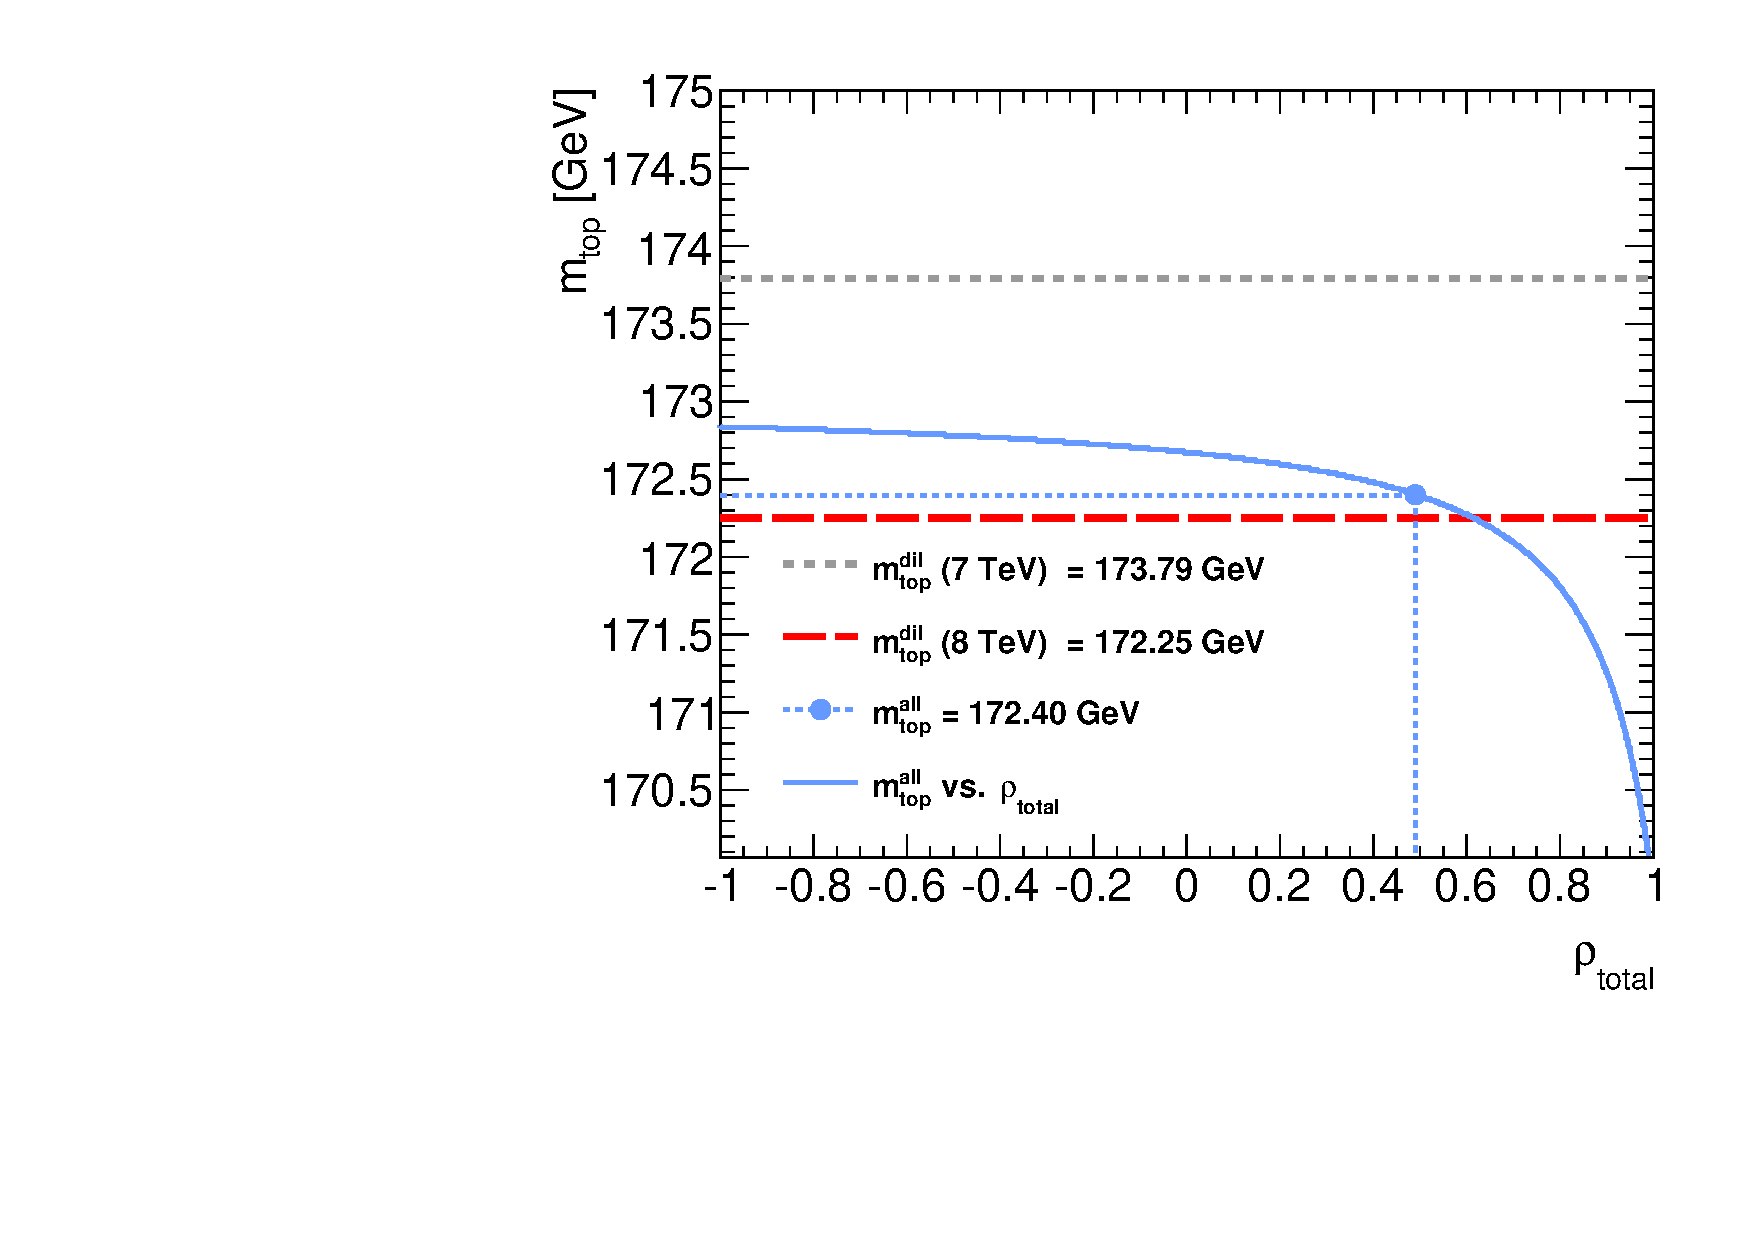
\includegraphics[width=0.49\textwidth]{./figs/fig_8TeV_TRC28_wp70/CombValRhoDep_8dil_7dil.pdf}
  \label{sfig:CombValRhoDep78Dil}
}
\subfloat[\Dil\ ($\sqrts=7$ and $8$~\TeV)]{
  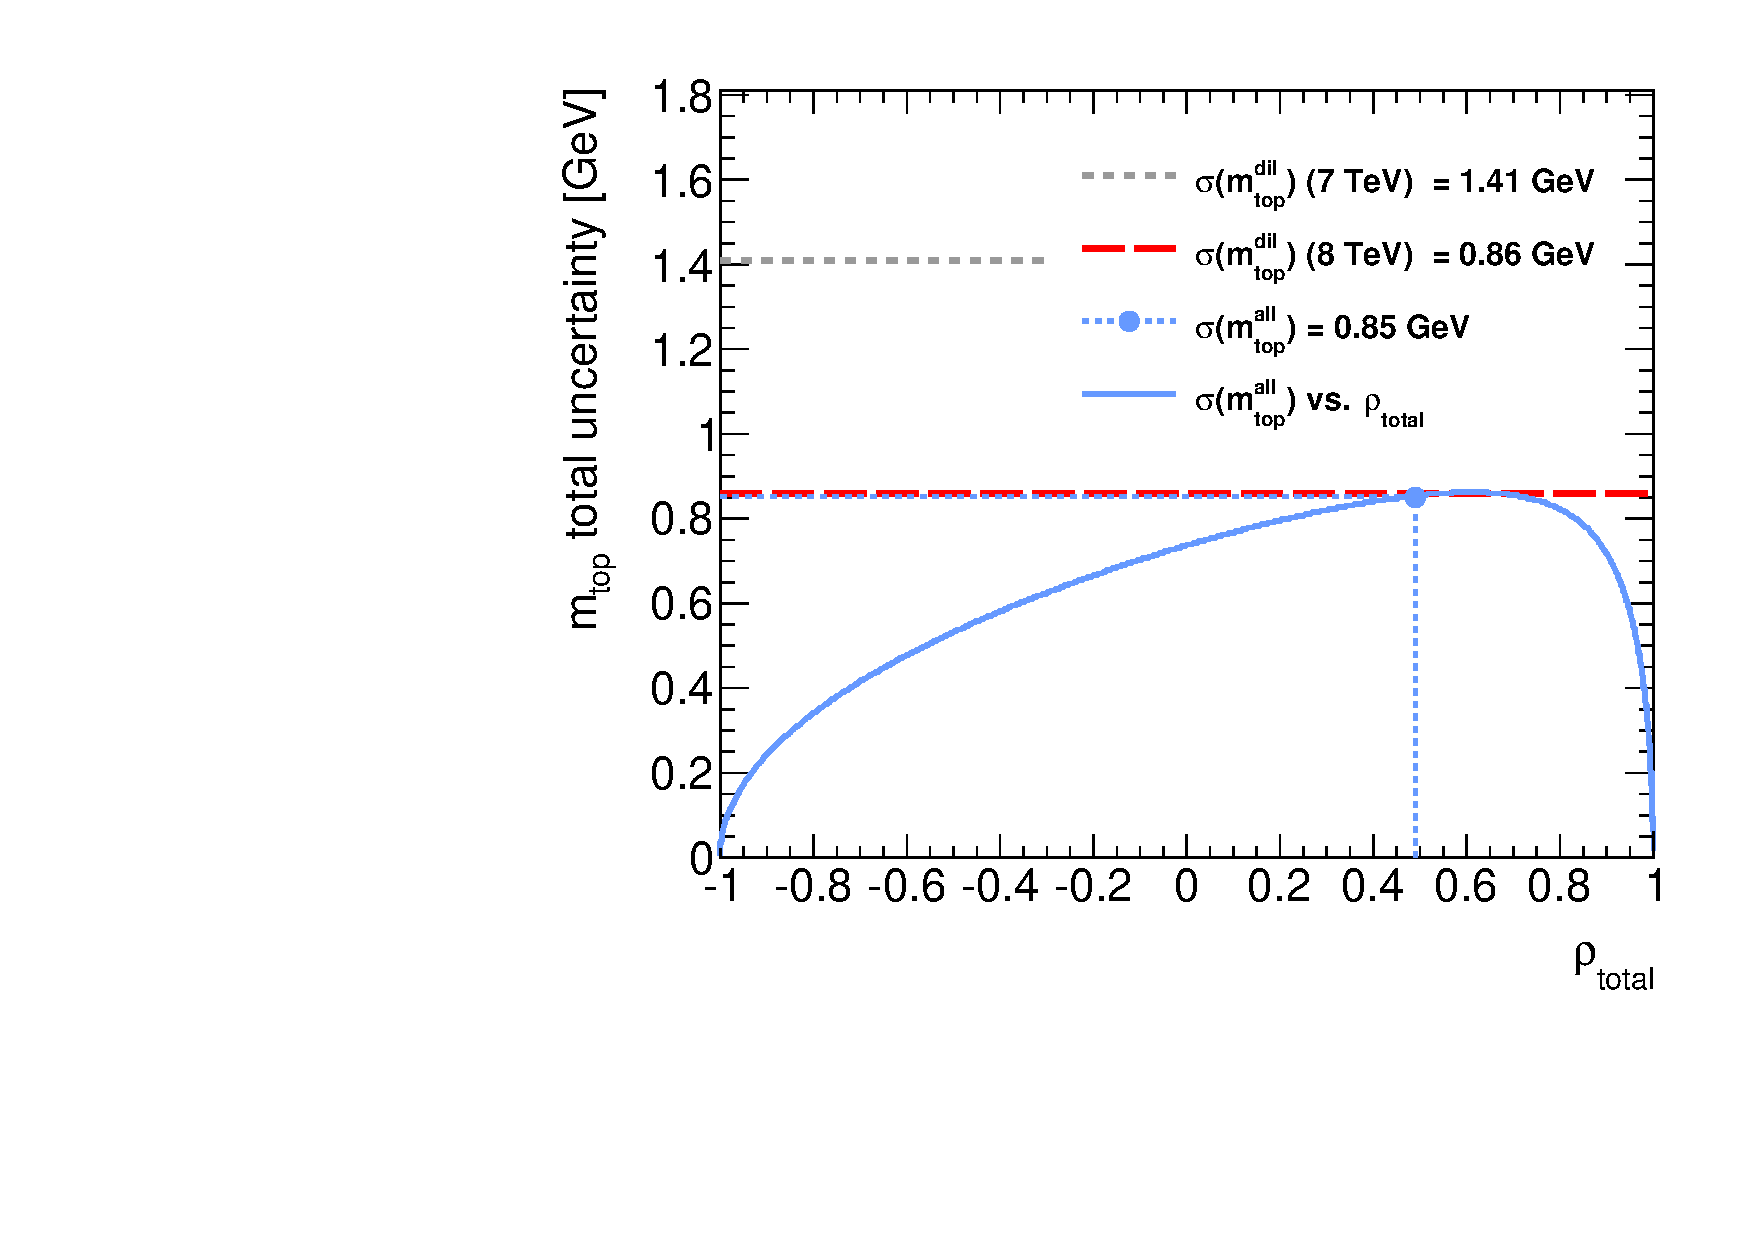
\includegraphics[width=0.49\textwidth]{./figs/fig_8TeV_TRC28_wp70/CombUncRhoDep_8dil_7dil.pdf}
  \label{sfig:CombUncRhoDep78Dil}
}
\hfill
\subfloat[\Dil\ ($\sqrts=8$~\TeV) and \ljets\ ($\sqrts=7$~\TeV)]{
  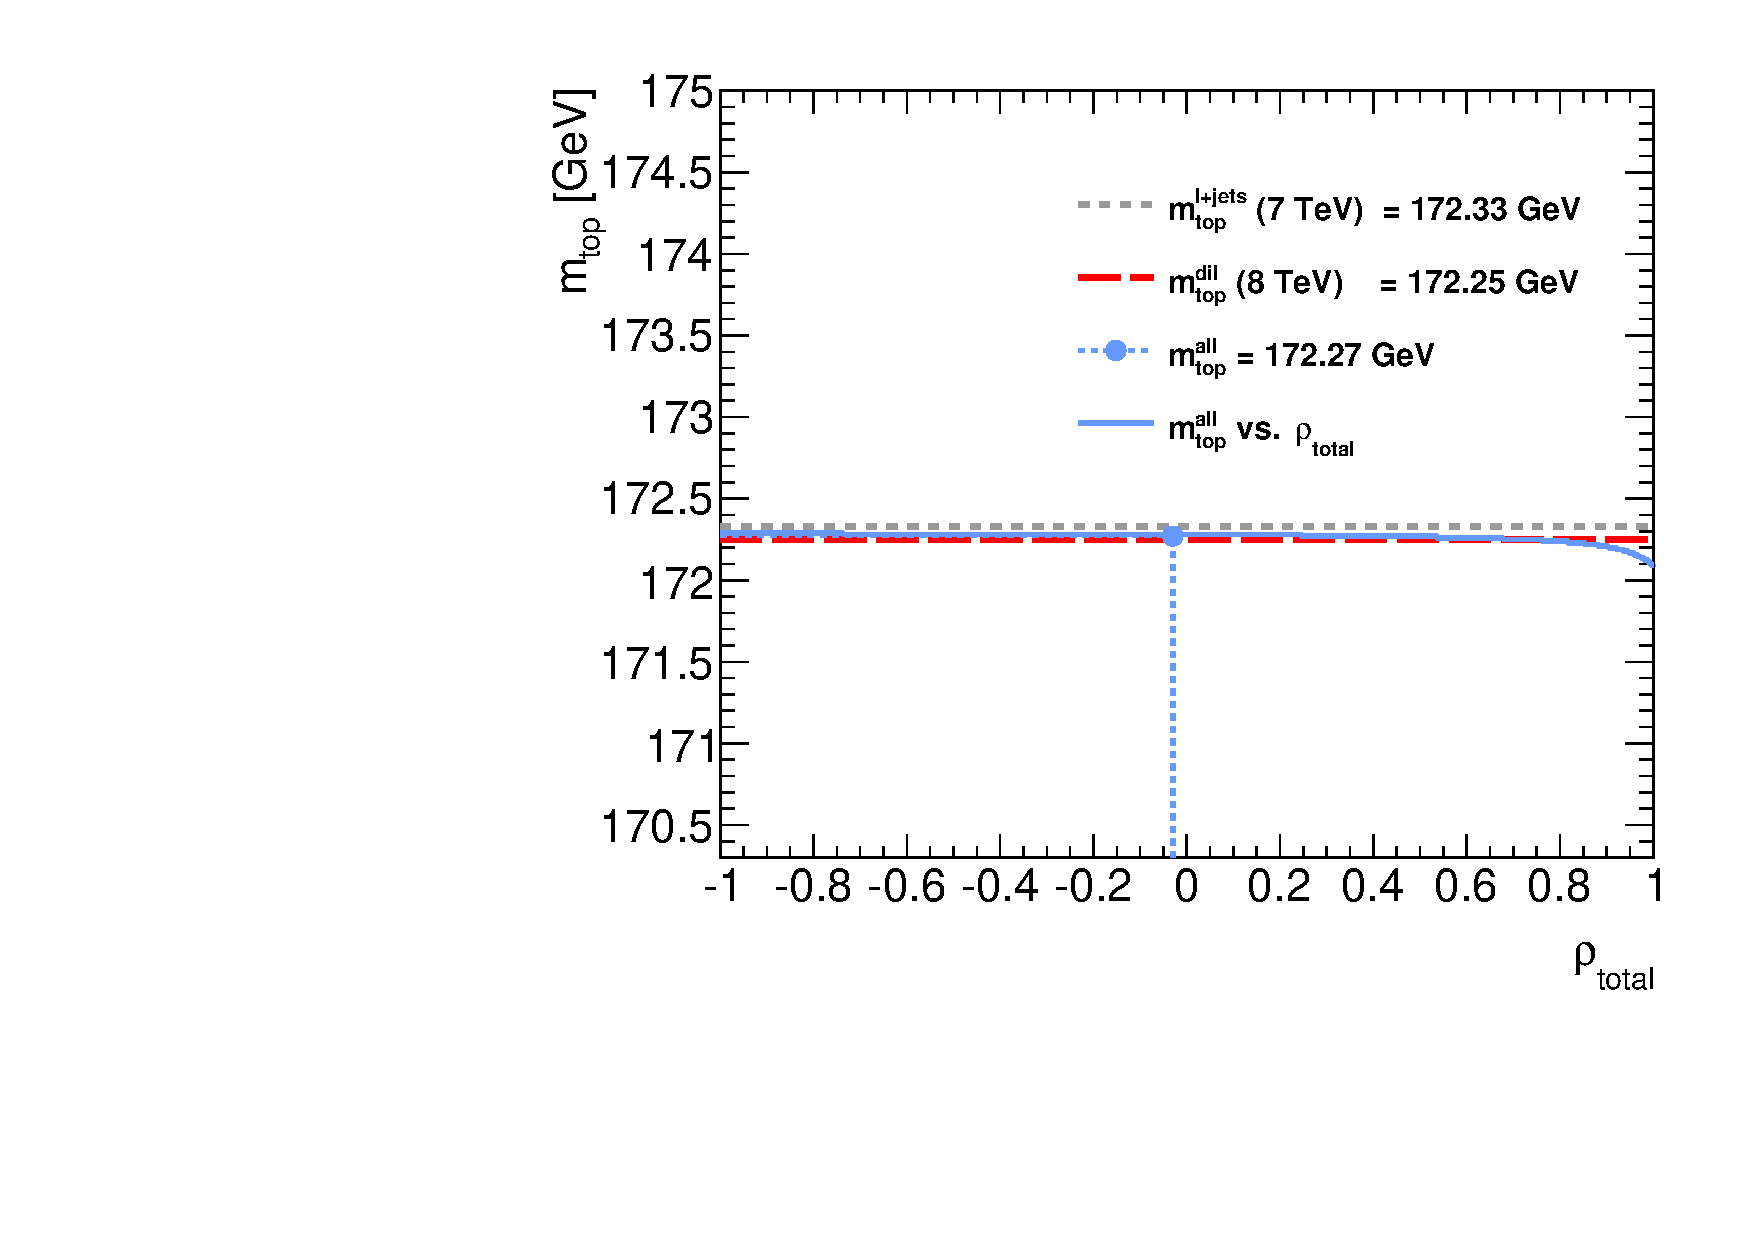
\includegraphics[width=0.49\textwidth]{./figs/fig_8TeV_TRC28_wp70/CombValRhoDep_8dil_7ljets.pdf}
  \label{sfig:CombValRhoDep7lj8dil}
}
\subfloat[\Dil\ ($\sqrts=8$~\TeV) and \ljets\ ($\sqrts=7$~\TeV)]{
  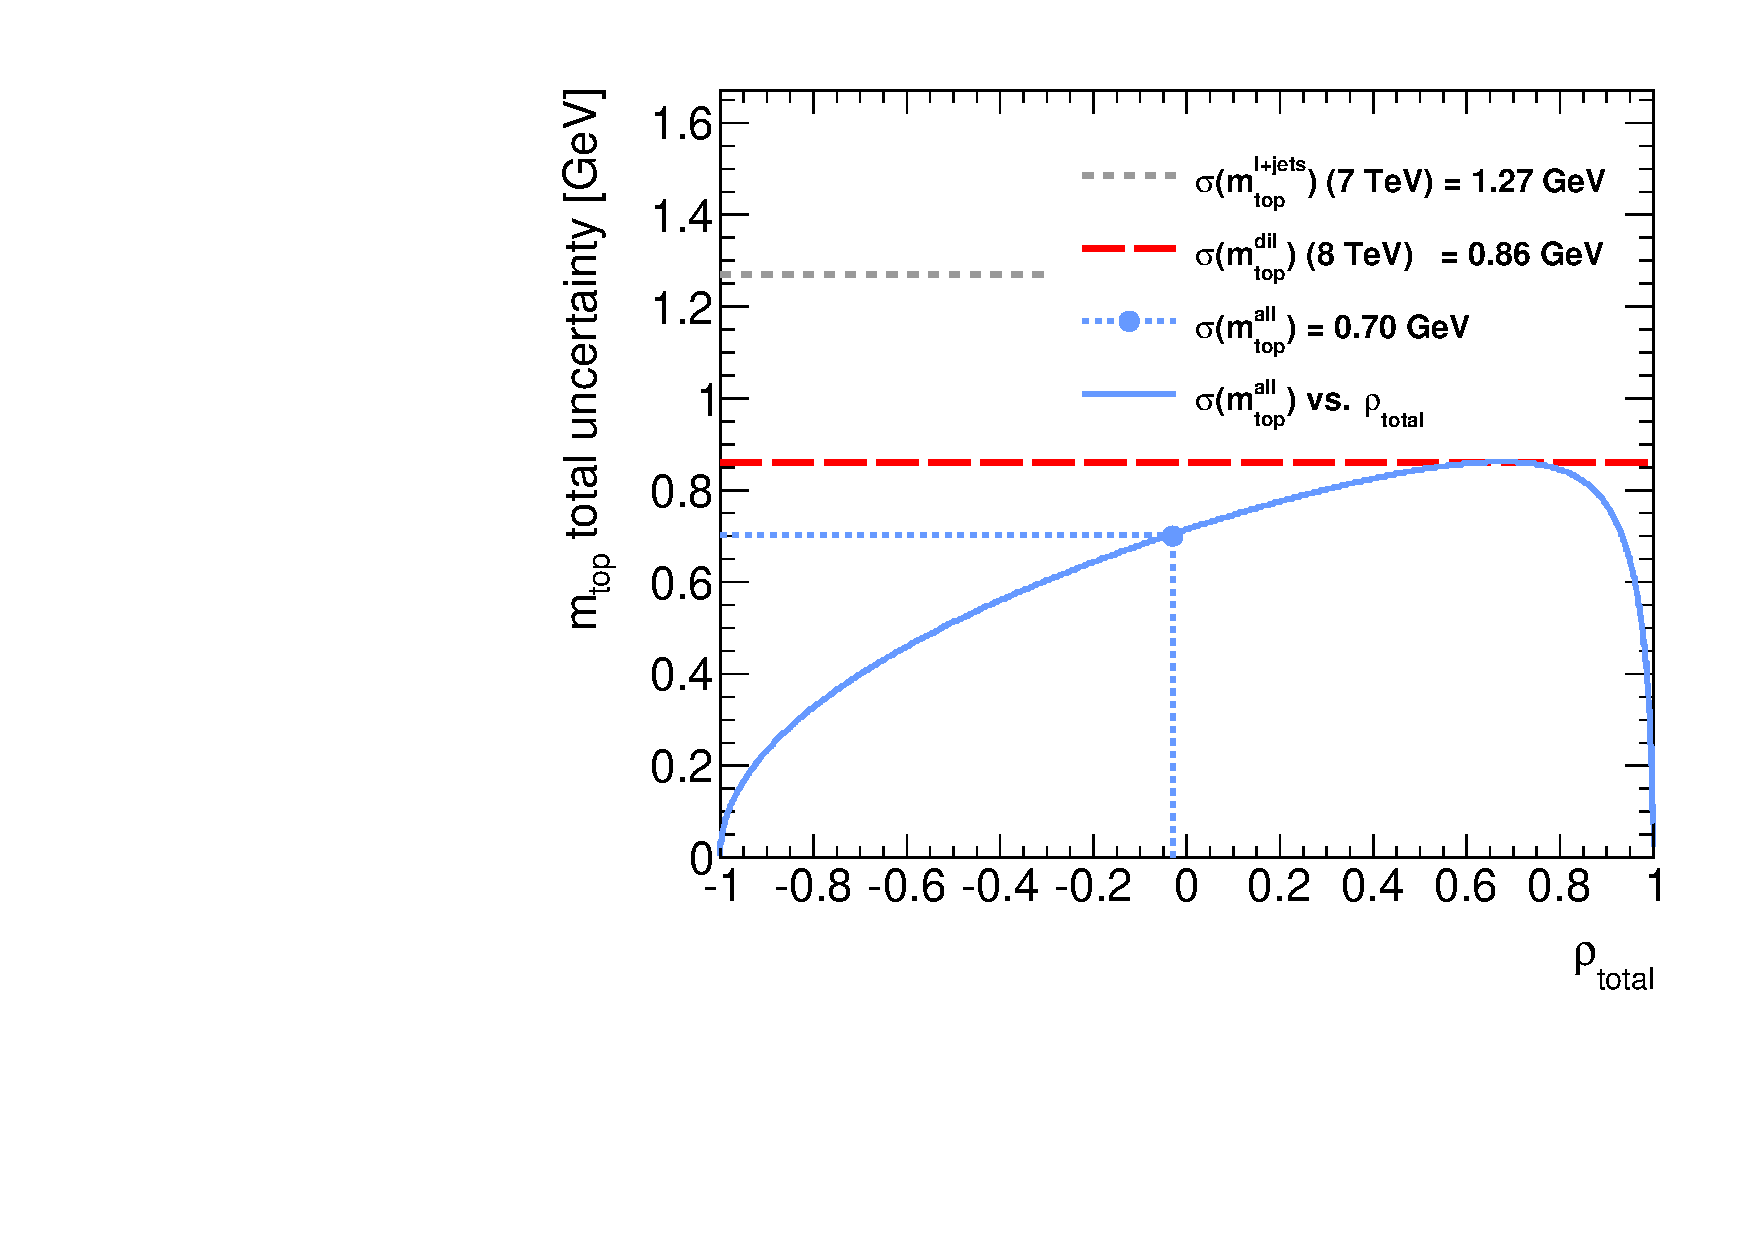
\includegraphics[width=0.49\textwidth]{./figs/fig_8TeV_TRC28_wp70/CombUncRhoDep_8dil_7ljets.pdf}
  \label{sfig:CombUncRhoDep7lj8dil}
}
\caption[Stability of the combination for the $\sqrts=7$ and $8$~\TeV\ analyses]{
%
The dependence of the central values (left) and the final uncertainties (right) of the combined result (blue) of the combination of the result at $\sqrts=8~\TeV$ in the \dil\ channel with the two results in the \dil\ (top) and \ljets\ channel (bottom) at $\sqrts=7~\TeV$ as a function of the total correlation. 
%
For comparison, the corresponding values for the input measurements are also shown (grey and red dashed lines).
%
  \label{fig:combinationrho78}}
\end{figure*}
%%%%%%%%%%%%%%%%%%%%%%%%%%%%%%%%%%%%%%%%%%%%%%%%%%%%%%%%%%%%%%%%%%%%%%%%%%%%%%%


The combined result for the two measurements in the \dil\ channel alone is $\mtdl = \XZ{\CombValueDL}{\CombStatDL}{\CombSystDL}~\GeV = \XZtot{\CombValueDL}{\CombTotDL}~\GeV$, providing only a \CombImprovementDL\ improvement with respect to the most precise single input measurement, i.e. the result at $\sqrts=8$~\TeV\ carrying a \gls{BLUE} combination weight of \CombWeightDLeightDL. This is a consequence of the measurement correlation of \CorrDil. The $\chi^2$ probability of the combination is \CombChiSqProbDL\ and variations of the input uncertainties and correlations yield a good stability of the central value and the combined total uncertainty. The corresponding distributions from 1000 pseudo-experiments are observed to be approximately Gaussian with a width of $\CombValueStabDL$ and $\CombTotStabDL~\MeV$, respectively. 
%
The same holds for the distribution of the determined correlation, which exhibits a width of \CorrDilUnc. 
%
The variation of the central value is larger than the ones observed for the other combinations, due to the increased correlation dependence of the central value, shown in \fig~\subref*{sfig:CombValRhoDep78Dil}. The resulting central value lies in a region of steeper slope and therefore the corresponding uncertainty is higher.
%
Using the the strong \gls{JES} correlation scenario yields negligible changes of $\CombValueStrongDiffDL$~\MeV\ on the central value and $\CombTotStrongDiffDL$~\MeV\ on the final uncertainty.
%
%%%%%%%%%%%%%%%%%%%%%%%%%%%%%%%%%%%%%%%%%%%%%%%%%%%%%%%%%%%%%%%%%%%%%%%%%%%%%%%%%%%%%%
\begin{figure*}[tbp!]
\centering
\subfloat[Distribution of the combined central values]{
  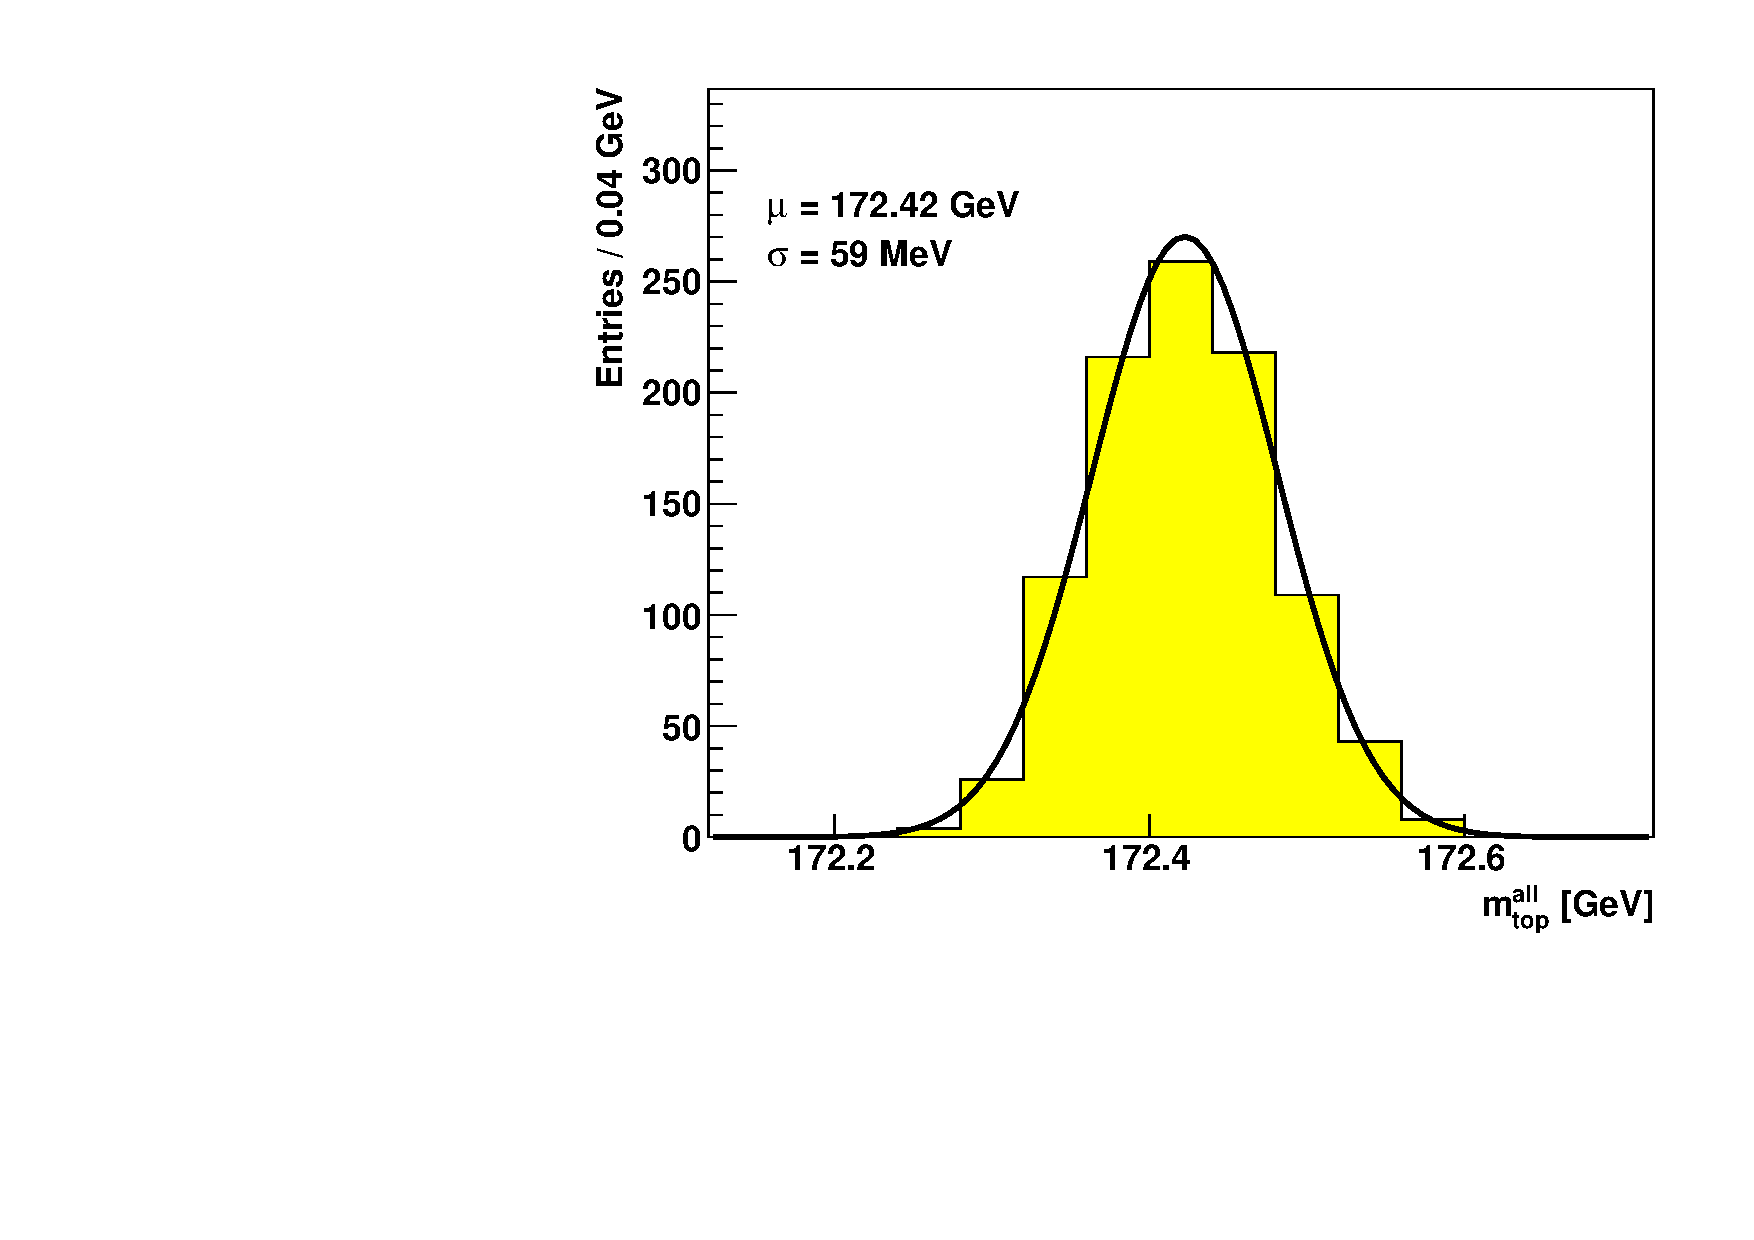
\includegraphics[width=0.49\textwidth]{./figs/fig_8TeV_TRC28_wp70/Combination_7_8TeV_stability_central.pdf}
  \label{sfig:combstabcentral}
}
\subfloat[Distribution of the combined uncertainties]{
  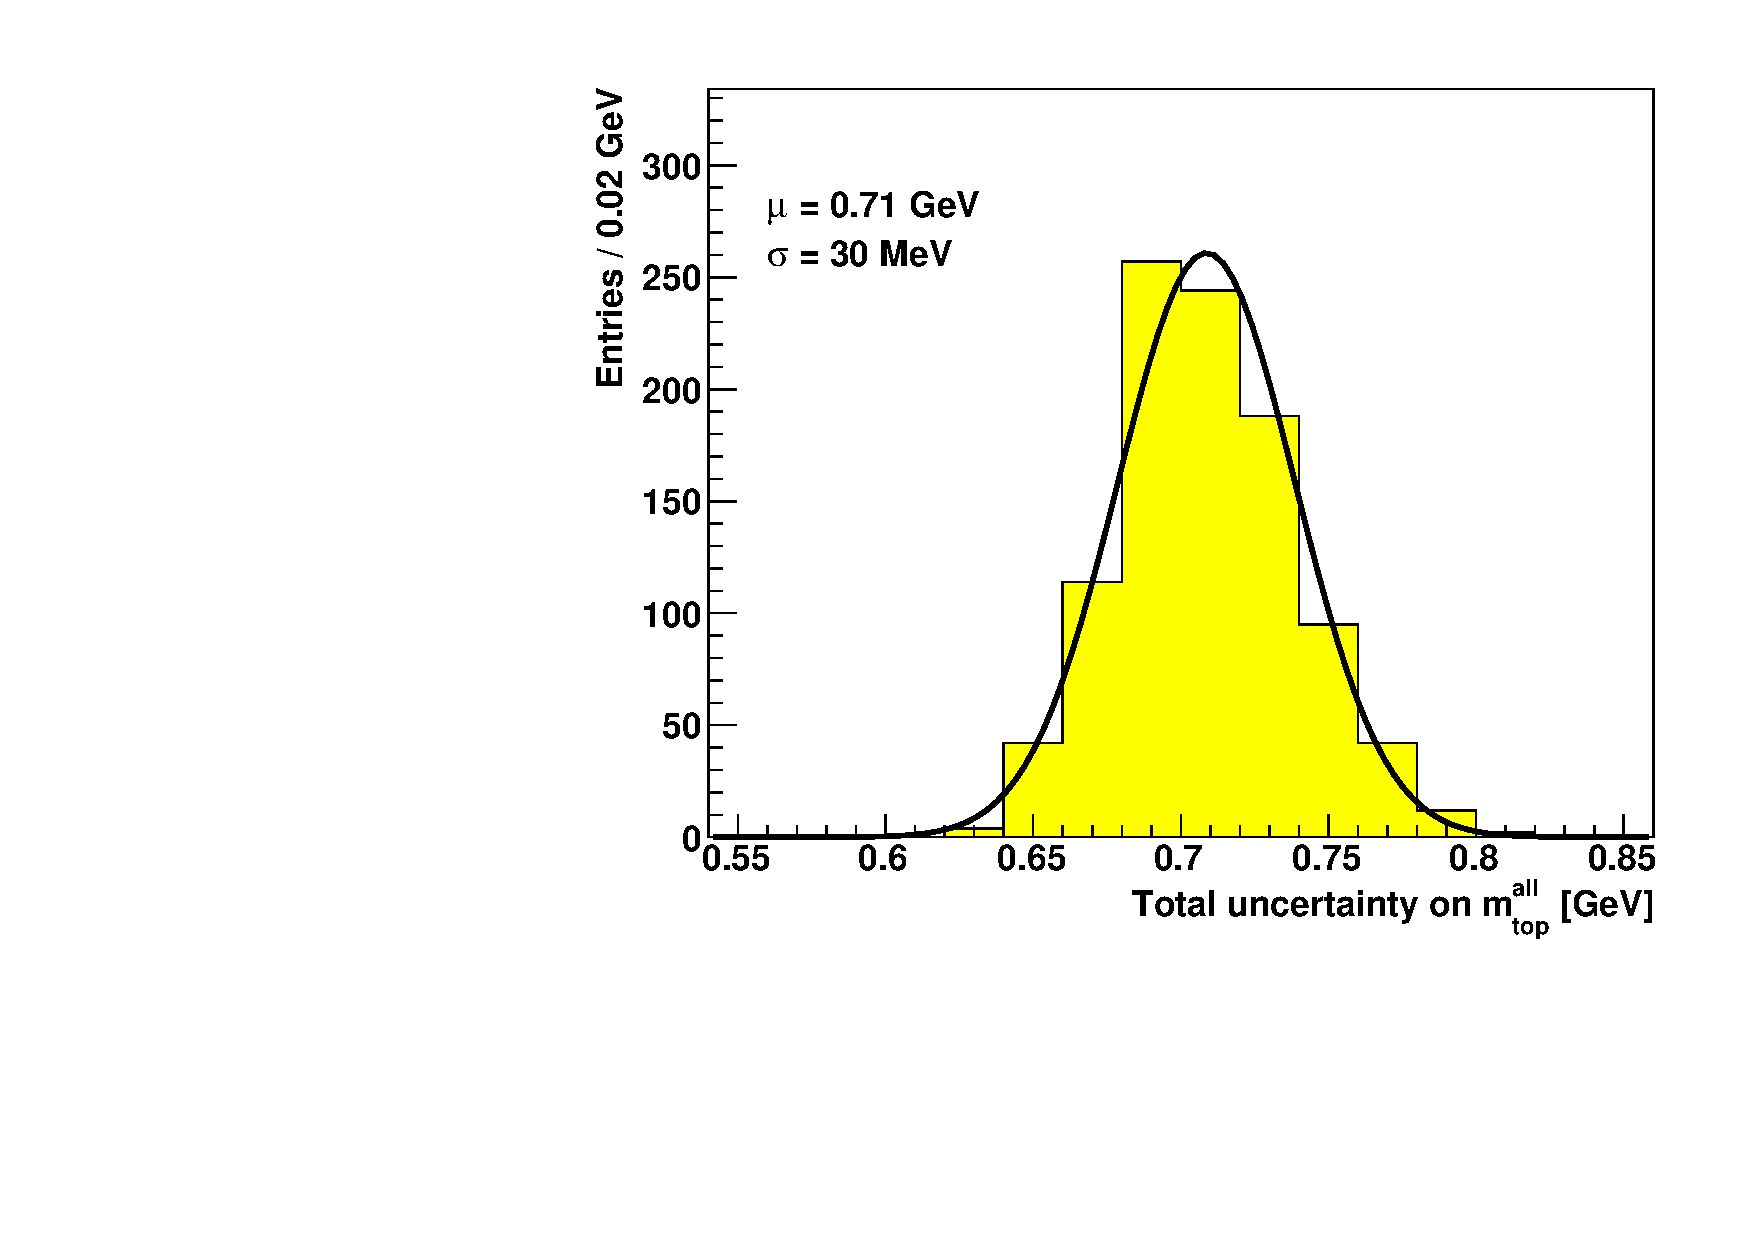
\includegraphics[width=0.49\textwidth]{./figs/fig_8TeV_TRC28_wp70/Combination_7_8TeV_stability_unc.pdf}
  \label{sfig:combstabunc}
}
\caption[Stability determination for the $\sqrts=7$ and $8$~\TeV\ analyses]{
%
The combination results of 1000 pseudo-experiments for the central value and the total uncertainty. For each of those, the size of the uncertainty and the correlation were newly evaluated, based on a random variation of each systematic uncertainty within its statistical precision. The parameters of the Gaussian function fitted to the distributions are shown as well.
%
\label{fig:combstab}
}
\end{figure*}
%%%%%%%%%%%%%%%%%%%%%%%%%%%%%%%%%%%%%%%%%%%%%%%%%%%%%%%%%%%%%%%%%%%%%%%%%%%%%%%%%%%%%%


The combination of all three measurements provides a \CombImprovement\ improvement with respect to the most precise single input measurement, which is the \ttbarll\ analysis at $\sqrts=8$~\TeV. The combined result is $\mtall = \XZ{\CombValue}{\CombStat}{\CombSyst}~\GeV = \XZtot{\CombValue}{\CombTot}~\GeV$. The central value and the combined total uncertainty are stable at the level of $\CombValueStab$ and $\CombTotStab~\MeV$, respectively. The combined central value and total uncertainty distributions of the corresponding pseudo-experiments are shown in \fig~\ref{fig:combstab}. Using the strong \gls{JES} correlation scenario yields changes of $\CombValueStrongDiff$~\MeV\ on the central value and $\CombTotStrongDiff$~\MeV\ on the final uncertainty. These effects are negligible, compared to the total uncertainty of the combined result and no additional systematic uncertainty is assigned. 
%
The $\chi^2$ probability of the combination is \CombChiSqProb\ and the \gls{BLUE} combination weights of the \ljets\ and \dil\ analyses at $\sqrts=7$~\TeV\ and the \dil\ analysis at $\sqrts=8$~\TeV\ are \CombWeightLLseven, \CombWeightDLseven\ and \CombWeightDLeight, respectively.
%
A variation of the blinded central value of the $\sqrts=8$~\TeV\ analysis in the combination, corresponding to the width $\sigma=0.5~\GeV$ of the Gaussian \gls{pdf} used for the blinding, yields a variation of $\Delta\mtall=^{+0.29}_{-0.29}$~\GeV. The unblinded result is likely to lie within this region.
%up 172.69
%down 172.11
%central 172.40








\section{Summary}
%
% A novel approach enables the evaluation of correlations related to systematic uncertainties for the first time, enabling the exploitation of the stabilising effect of anti-correlations of measurements. 
%
For the first time in \mt\ combinations, the correlations of the measurements have been evaluated rather than assigned based on physics arguments~\cite{Aad:2015nba}. By carefully designing the analysis methods in the different decay channels, the estimators are anti-correlated for a number of uncertainty sources that significantly contribute to the total systematic uncertainty. By construction, this leads to much larger improvements with respect to the the most precise measurement in the combination, than what is usually achieved with assigned correlations, which are frequently larger than the evaluated ones.



The combination of the \mt\ measurements in the \ttbarll\ and \ttbarlj\ channels at $\sqrts=7$~\TeV\ yields $\mtcb = \XZtot{172.99}{0.91}~\GeV$, constituting a relative precision of $0.5\%$. This corresponds to a 28\% precision gain, compared to the most precise input measurement, and a 22\% precision gain compared to the traditional correlation scenario.




Using a dedicated mapping of uncertainty categories, the combination of the two $\sqrts=7$~\TeV\ measurements with the $\sqrts=8$~\TeV\ measurement in the \dil\ channel has been performed. The combination yields a \tquark\ mass of $\mt = \XZ{\CombValue}{\CombStat}{\CombSyst}~\GeV = \XZtot{\CombValue}{\CombTot}~\GeV$, corresponding to a relative precision of $0.4\%$.
%
The combination is mostly limited by the calibration of the jet energy scales and the MC modelling of \ttbar\ events. 
%
The inclusion of the \mt\ measurement at $\sqrts=8$~\TeV\ in the \ljets\ channel in the combination is expected to yield another significant improvement in precision due to the anti-correlations that are present by construction. This analysis is currently being finalised and results are expected soon.
%
%this is speculation, says Giorgio:
% The general trend of decreasing experimental uncertainties, which is driven by the ever improving detector calibration and statistical power provided by the \gls{LHC}, will eventually lead to dominating theoretical uncertainties. 
% %
% These are not trivial to control by the analyser and will require increased efforts in the theoretical understanding of high energetic particle collisions.



